%!TEX root = ../main.tex

\chapter{Systematic review}
\label{ch:2}

With the literature doubling in size since the last review on MECs, it has become increasingly difficult to gain a broad and integrated understanding of the empirical and theoretical research on the subject. Notably, crucial questions remain about the criteria that are necessary and sufficient to characterise MECs. In this chapter, we systematically review the literature on MECs in order to reconcile diverging opinions and empirical findings on their psychological nature, and to develop a preliminary model that provides a robust framework for future hypothesis-driven research. We explore the context behind current research on MECs, discuss how they relate to emotional and aesthetic responses, assess current empirical measures and paradigms, summarise their physiological and neural correlates, categorise their possible stimulus-driven elicitors, examine how they are affected by individual differences, and evaluate theoretical perspectives about their potential evolutionary causes. We conclude by providing a preliminary model of MECs that suggests different pathways for the experience of MECs, a dataset listing pieces of music reported to elicit MECs in the reviewed literature, and a set of open issues, hypotheses, and recommended approaches for future research.

\section{Introduction}
\label{se:rev-intro}

The knowledge base on MECs is rapidly expanding, and as research findings accumulate, it is becoming increasingly difficult to gain a comprehensive and integrated psychological picture of what MECs entail. Notably, crucial questions remain about the criteria that are necessary and sufficient to characterise MECs.

Frequently cited papers describe MECs as ``a spreading gooseflesh, hair-on-end feeling that is common on the back of the neck and head and often moves down the spine'' \parencite[p. 173]{panksepp1995}, ``a particularly intense, euphoric response to music [frequently accompanied] by an autonomic or psychophysiological component'' \parencite[p. 11818]{blood2001}, ``intense emotional experiences involving sensations such as goose bumps or shivers down the spine'' \parencite[p. 131]{koelsch2010}, or ``a pleasant tingling feeling associated with the flexing of hair follicles, resulting in gooseflesh (technically called piloerection) accompanied by a cold sensation, and sometimes producing a shiver'' \parencite[p. 591]{huron2010}.

While superficially similar, these definitions provide pointers to crucial questions which need to be addressed. If MECs are to be used as an indicator of pleasurable experiences, it is important to understand how universal and frequent they are, as well as the nature of their relationship with emotional and aesthetic responses, in order to assess whether or not their relevance is justified, and, if so, clarify their underlying psychological mechanisms. The phenomenology of MECs also deserves clarification, as it is unclear whether empirical findings refer to a single psychophysiological response or to distinct experiences with little common ground. The specificity of the physiological and neural signatures of MECs needs to be explored to establish whether MECs invoke general-purpose mechanisms involved in other functions, such as emotional processing and reward, or are distinguishable from these experiences. Finally, it is necessary to investigate the causes of MECs, both in terms of stimulus-driven properties and individual differences, to better understand their origin, and thereby achieve a broader and more integrated understanding of the empirical and theoretical research on MECs.

MECs are often mentioned in the literature on music and emotion, but at the time of writing, there are only three short reviews entirely dedicated to MECs \parencite{grewe2009b, harrison2014, mori2014a}, one review about MECs and the autonomous sensory meridian response \parencite{delcampo2016}, one review about MECs and music therapy \parencite{tihanyi2016}, one philosophical essay about MECs and musical aesthetics \parencite{levinson2006}, two book chapters discussing MECs within the context of musical expectation \parencite{huron2010} and of the evolutionary basis of music \parencite{altenmuller2013}, and book chapters on music and emotion which contain subsections on MECs \parencite[e.g.,][]{corrigall2013, corrigall2015, hodges2016, hunter2010, juslin2019, mcdermott2012, sachs2018, stark2018, vuust2010}.

Despite referring to the same phenomenon, as evidenced by the fact that these contributions all make reference the same seminal papers on MECs \parencite{blood2001, goldstein1980, panksepp1995, sloboda1991}, the topics listed above are very diverse, once again illustrating the need for a clear integration of the 40 years of available research on MECs. The purpose of this chapter is therefore to systematically review the literature on MECs in order to reconcile diverging opinions and empirical findings on their psychological nature, and to develop a preliminary model that provides a robust framework for future hypothesis-driven research.

\section{Methods}
\label{se:rev-methods}

We performed a systematic literature search in order to ensure comprehensive coverage. We opted to conduct a systematic review instead of a meta-analysis because of the great diversity of topics and methods in research on MECs, which results in insufficiently comparable research evidence for a quantitative aggregation of empirical findings. We first outline the search procedure, before going over the inclusion and exclusion criteria, and finally describing how the findings are organised in the next sections of the present chapter.

\subsection{Literature search}

We searched the databases Web of Science, APA PsycInfo and PsycExtra, PubMed, Scopus, and Google Scholar, using a cut-off date of 30 April 2020, for articles, reviews, conference papers, books, book chapters, and doctoral dissertations about chills and music. All contributions containing the term \emph{music} and at least one of \emph{chills}, \emph{thrills}, \emph{frisson}, \emph{shivers}, \emph{goosebumps}, or \emph{piloerection} were considered, resulting in 149 records being identified on Web of Science, 85 records on APA PsycInfo and PsycExtra, 47 records on PubMed, and 127 records on Scopus. We also examined the first 100 records returned by Google Scholar for the same search terms, as well as the first 100 records on Google Scholar for contributions dated 2019 or later to ensure we did not miss recent contributions. This process resulted in the identification of 346 unique records.

\subsection{Inclusion and exclusion criteria}

The objective was to include all publications about MECs. We therefore included contributions written in any language, as long as they mentioned both chills and music. The first exclusion criterion accounted for the fact that the queried terms are commonly used in the English language, and therefore appear in many publications which are not about MECs. As a result, 117 irrelevant records were excluded. The second exclusion criterion accounted for the fact that MECs are often briefly mentioned to provide context in broader studies, reviews, or book chapters about music and emotion. As a result, 78 records containing no substantial information about MECs were excluded. In addition, we excluded five records that could not be retrieved, one article written in Japanese that could not be translated online due to issues with character encoding, one corrigendum, the content of which was already reflected in the associated publication, one editorial which simply listed the topics covered in a specific journal issue, and six records because the presented results were also fully covered in subsequent journal articles that were retained in the search. Finally, we included 30 articles and book chapters obtained through backward and forward reference searching, resulting in a total of 167 contributions which represented, to our knowledge, all the available academic literature on MECs.

\subsection{Organisation of findings}

The literature doubled in size since the reviews by \textcite{harrison2014} and \textcite{mori2014a}---in the present chapter, we reviewed 83 contributions about MECs dated 2014 or prior, and 84 contributions dated 2015 or later (see \autoref{fig:rev-1} for the yearly publication count).

\begin{figure}[t!]
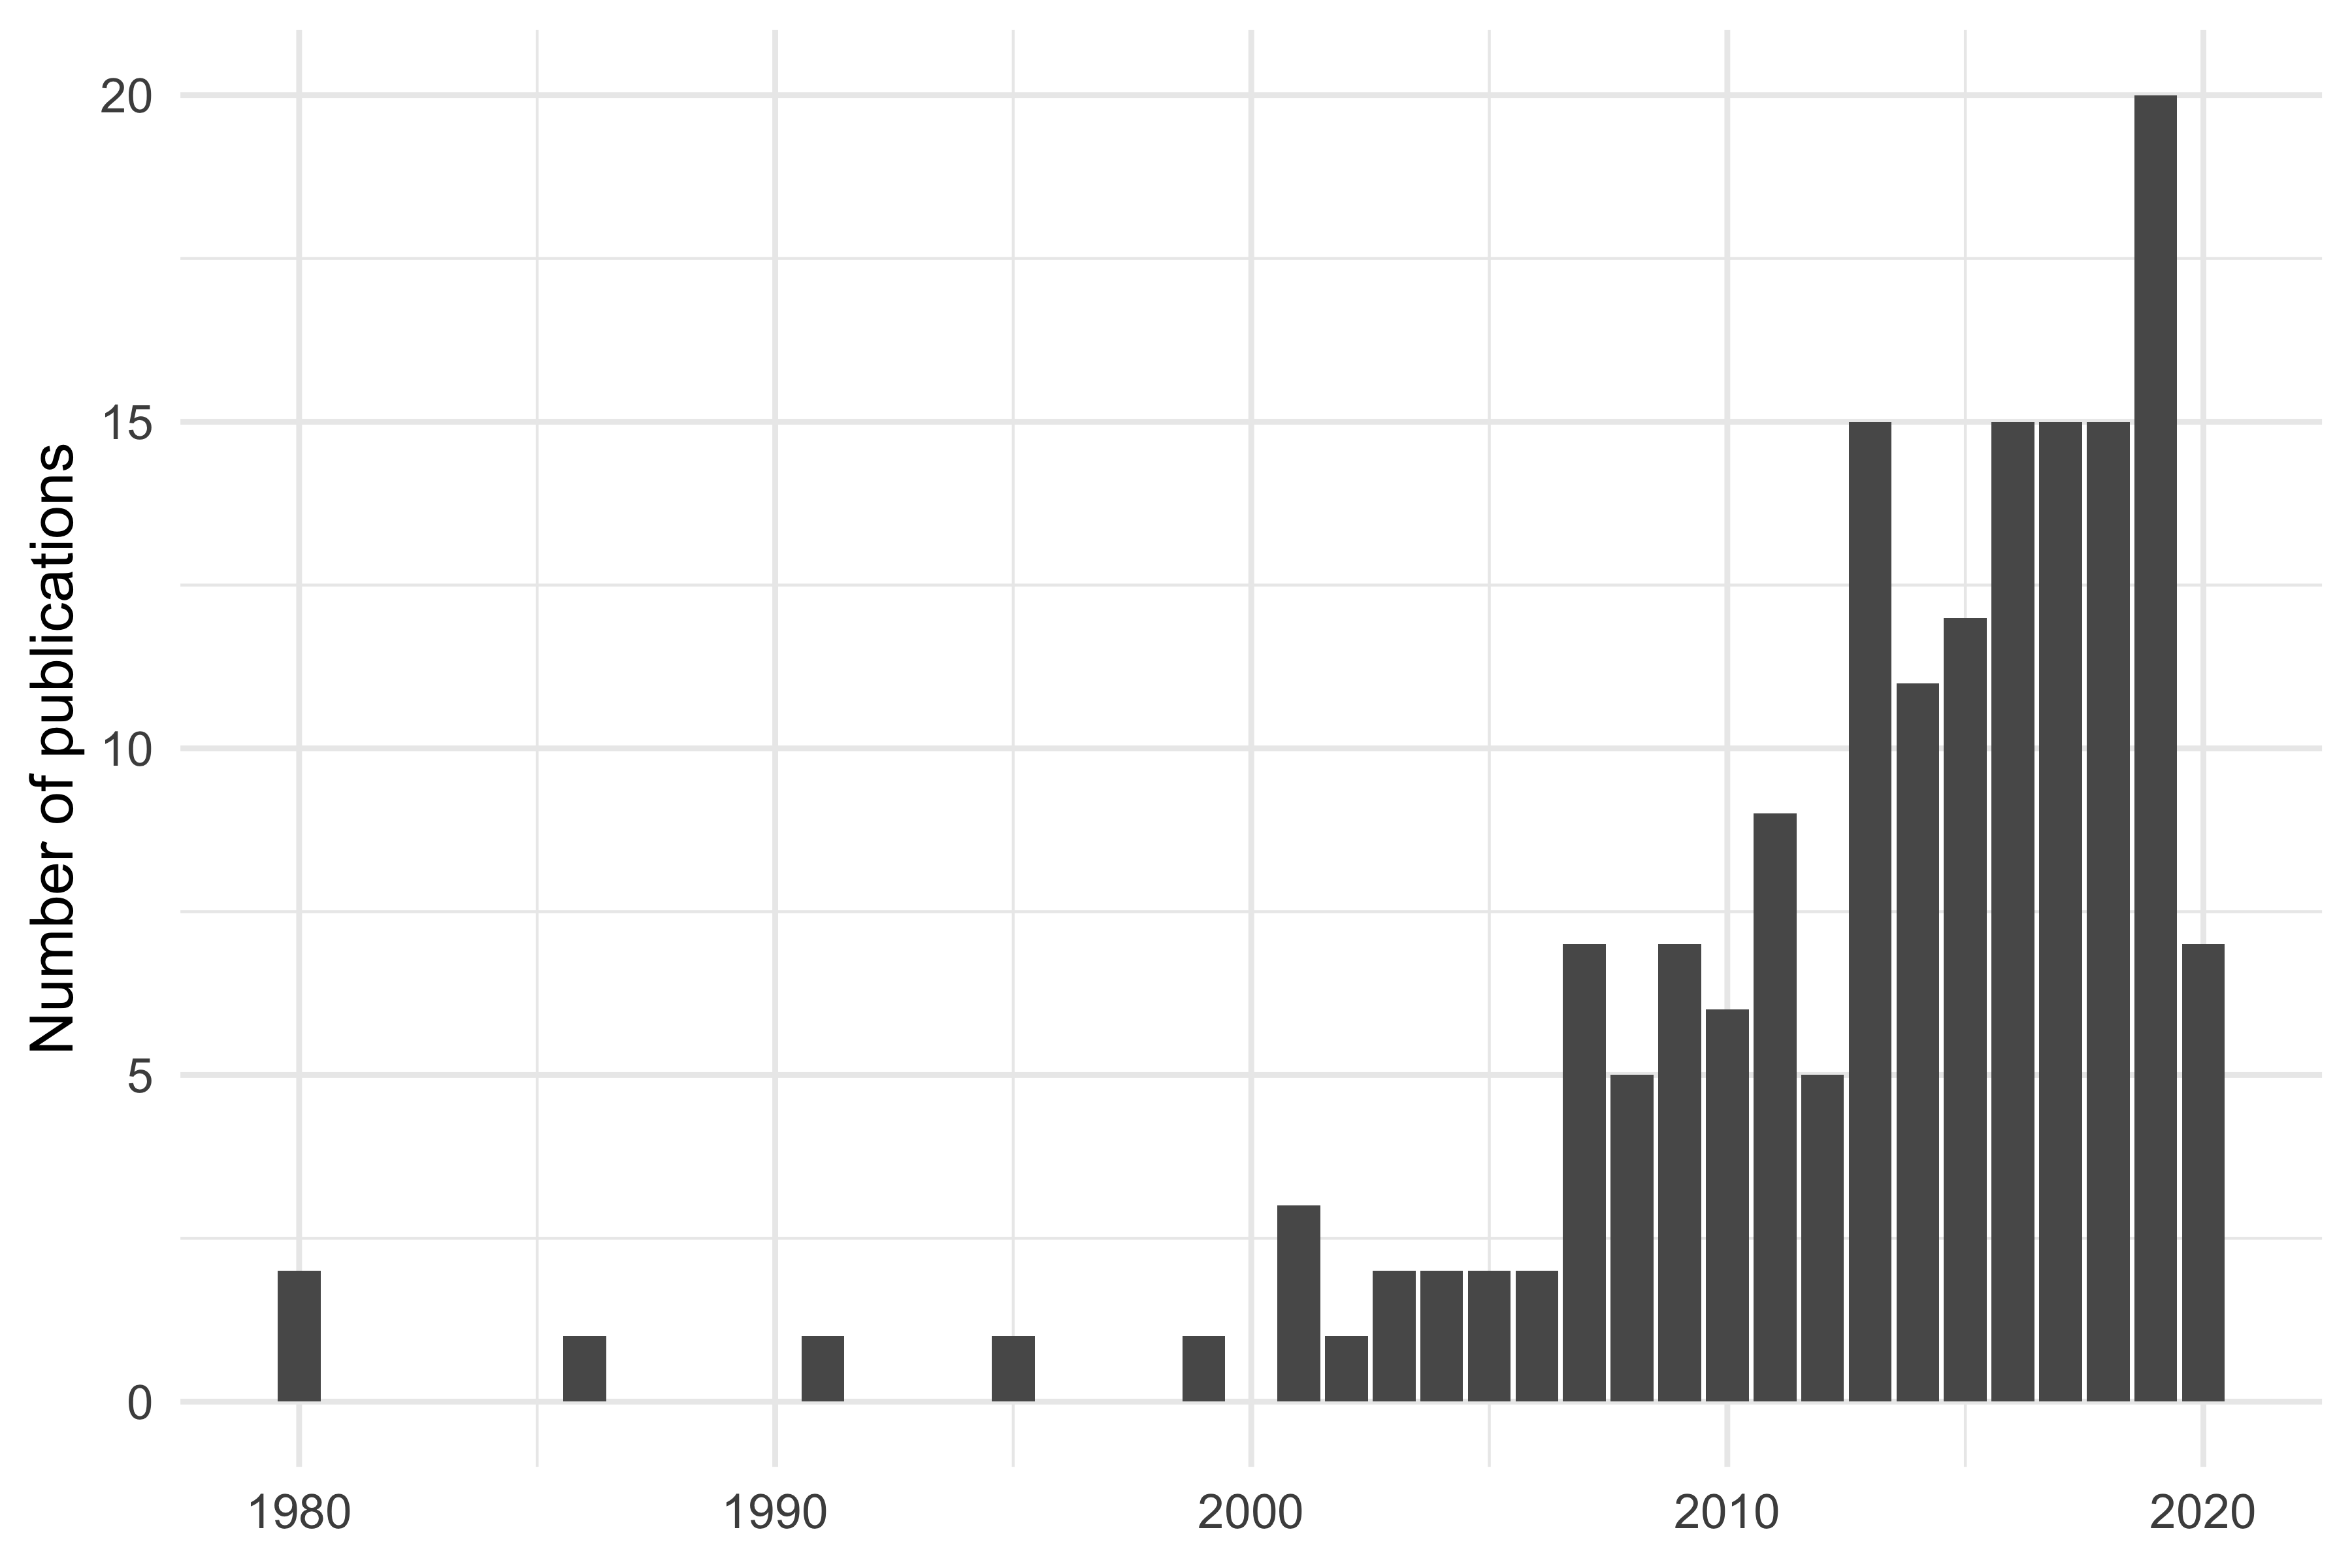
\includegraphics[width=\textwidth]{rev-1.png}
\centering
\caption{Yearly publication count for research on the topic of MECs reviewed in this chapter.}
\label{fig:rev-1}
\end{figure}

The vast majority of publications on MECs contain findings that pertain to several domains of interest, which logically emerged as empirical and theoretical findings were extracted from each reviewed study. As a consequence, instead of attempting to allocate the publications themselves to meaningful units, we distributed all of their findings across several overarching categories corresponding to these domains, therefore allowing broad and integrative coverage of the most pertinent and widely researched topics in research on MECs. The results are therefore structured as follows. Sections \ref{se:rev-results-1}, \ref{se:rev-results-2}, and \ref{se:rev-results-3} consider the wider context within which empirical and theoretical research on MECs has been conducted. We begin in Section \ref{se:rev-results-1} by considering terminological issues, the phenomenological nature of MECs, their prevalence and frequency, and their relationship with other psychological processes. In Section \ref{se:rev-results-2}, we expand on the nature of the relationship between MECs, pleasure, and emotional and aesthetic experience, before assessing subjective and objective ways of measuring MECs, as well as experimental paradigms used in research on MECs in Section \ref{se:rev-results-3}. In the subsequent sections of the chapter, we review the empirical literature on the biological basis of MECs, considering associations between MECs, arousal, and physiological responses (Section \ref{se:rev-results-4}), and neural correlates of MECs in the basal ganglia and other brain structures (Section \ref{se:rev-results-5}). We then turn to theoretical considerations regarding the causes of MECs. We review the empirical literature to identify the stimulus-driven causes of MECs and categorise them into acoustic, musical, and emotional elicitors (Section \ref{se:rev-results-6}), examine empirical effects of individual and personality differences on the occurrence of MECs (Section \ref{se:rev-results-7}), and critically evaluate the degree of support provided by the reviewed evidence for current theories on the function of MECs (Section \ref{se:rev-results-8}). These findings are summarised and expanded upon in the discussion, and the quality of the reviewed research is evaluated, after which we conclude by providing a preliminary model of MECs, a dataset listing pieces of music reported to elicit MECs in the reviewed literature, and a set of hypotheses and recommendations for future research.

\section{Results}
\label{se:rev-results}

\subsection{Context}
\label{se:rev-results-1}

A significant amount of research has focused on identifying exactly what MECs are, but there remains uncertainty about many of their defining aspects. In this section, we review the terminology associated with MECs, their phenomenological nature, their prevalence and frequency, and their relationship with other psychological processes, including emotional and aesthetic responses to music.

\subsubsection{Terminology}

Besides definitions of MECs, an initial source of confusion is the broad range of terms used to refer to the phenomenon. Terms such as musical chills, aesthetic chills, art-elicited chills, shivers, shivers down the spine, psychogenic shivering, thrills, frisson, goosebumps, gooseflesh, goose pimples, piloerection, emotional piloerection, hair standing on end, and skin orgasm, have been used interchangeably over the years, and there is no explicit consensus as to which option should be preferred. \textcite{harrison2014} recommended the use of \emph{frisson}, a term first used in the context of research on MECs by \textcite{huron2006} and \textcite{levinson2006}, which has the advantage of providing a relatively nonspecific way to describe an emotional response with a physiological component, while avoiding the burden of cultural associations present in other terms. While this is a sound recommendation, the term \emph{frisson} is sparsely used in the literature. We would argue that the need for a unified term of reference outweighs considerations about the colloquial use of the term, and therefore recommend the use of \emph{chills}\footnote{Following common usage in the literature, we use the word ``chills'' as a plural-only, non-countable noun, like clothes or groceries. We feel this is consistent with the difficulty of identifying exactly what would constitute an individual chill (or a definite number of chills) and find it more natural to refer, for example, to an episode of chills.}, which has quite clearly become the most prevalent term in the recent literature. In the present thesis, we use \emph{chills} (for the psychophysiological response) and \emph{piloerection} (for goosebumps specifically) throughout, except when referring to specific findings from authors who used several terms in a single publication.

\subsubsection{Phenomenology}

Regardless of the terminology used, it is important to have a clear and consistent conception of the nature of MECs. This would ensure that participants in research on MECs provide responses about the same psychophysiological phenomenon. Failing to do so might lead to inconsistent empirical findings, making interpretation problematic and creating difficulties in relating empirical results between studies. However, identifying a clear and consistent phenomenological description of MECs is not straightforward in the existing literature. \textcite{goldstein1980} provided a thorough starting point through a series of unstructured and structured questionnaires, in which several groups of participants were asked to describe their experience of MECs. The results characterised MECs as a transient, pleasurable response associated with sudden changes in mood or emotion, commonly experienced by a large proportion of the population, and originating primarily in the upper spine or back of the neck, with other common points of origin being shoulders, lower spine, and scalp. Intense occurrences of MECs were described as longer in duration, and radiating to other body areas (most commonly the scalp, arms, shoulders, spine, and face). There are further, varying reports of the location from which MECs originate. The back (or spine), head (or scalp, face, or neck), and arms are the most commonly reported points of origin \parencite{craig2005, goldstein1980, neidlinger2017, panksepp1995, wassiliwizky2015}, with occasional mentions of hands or fingers \parencite{craig2005}, as well as legs \parencite{wassiliwizky2015}.

Interestingly, \textcite{craig2005} made the distinction between points of origin for shivers or tingling (listed above) and piloerection, which was most often reported to begin on the arms, back of the neck, or legs. This raises the important question of whether piloerection should be considered as an integral component of MECs or not. Again, opinions differ. While some definitions of MECs suggest that piloerection is required \parencite{huron2010, panksepp1995}, most do not \parencite[e.g.,][]{blood2001, goldstein1980}, and empirical findings support the latter view. In self-reports, piloerection is often reported to happen less often than MECs \parencite{gabrielsson2011, silvia2011, sloboda1991}. In experimental settings, piloerection was only observed in 57\% \parencite{craig2005}, 40\% \parencite{benedek2011}, 43.1\% \parencite{sumpf2015}, and 40.7\% \parencite{wassiliwizky2017b} of participants who reported MECs. Seemingly, not all MECs involve piloerection \parencite{craig2005}, although most \parencite{benedek2011} or all \parencite{craig2005} occurrences of piloerection were found to happen during experiences of MECs. It is therefore likely that MECs, as reported by participants, do not always involve piloerection, although it is possible that experienced MECs might require an intensity threshold to be reached before piloerection can be observed \parencite{sumpf2015}, or that current piloerection detection methods are simply not accurate enough (for an overview of available methods, see Section \ref{se:rev-results-3}). While relying on self-reported or observed piloerection to study MECs is tempting, due to the objectivity it provides, it seems more appropriate at this stage to combine such an approach with self-reports of MECs \parencite[e.g.,][]{wassiliwizky2017b}, in order to avoid biasing research away from what people actually experience as MECs \parencite{maruskin2012}.

\subsubsection{Prevalence and frequency}

While 79\% of the 249 participants who completed Goldstein’s (\citeyear{goldstein1980}) questionnaires reported having experienced MECs in the past, additional figures about the prevalence of the ability to experience MECs are available in the literature: 90\% of a sample of 83 respondents for experiencing shivers down the spine at least once in the past five years \parencite[also reporting 62\% for goose pimples and 31\% for trembling]{sloboda1991}, over 80\% of 186 respondents for experiencing shivers down the spine or goose pimples at least rarely over the past five years \parencite{mlejnek2013}, or 86\% of 828 respondents for experiencing MECs with some regularity \parencite{panksepp1995}. In a survey of 196 people by \textcite{nusbaum2011}, 8\% of respondents never or rarely experienced MECs, and in a survey of 188 people by \textcite{silvia2011}, 11.2\%, 9.6\%, and 23.5\% never or rarely experienced chills down the spine, goosebumps, and feeling hair standing on end, respectively, although it is worth keeping in mind that for the latter study, only half of the reports were about experiences when listening to music. There are further figures available in the literature, showing MECs as generally less prevalent in experimental settings \parencite[e.g.,][]{colver2016, grewe2009a, konecni2007b}, but when looking at prevalence, it makes sense to consider only results from surveys of a reasonably representative sample of the population, since participants in lab experiments have most often been recruited for their ability to experience MECs, but might also not have been able to experience MECs under experimental conditions for a variety of reasons. Limitations remain, due to the fact that people interested in taking surveys about reactions to music might not be fully representative of the population, but from these results, it is reasonable to assume that 90\% is an upper limit for the proportion of the population that has the ability to experience MECs. Interestingly, when providing free reports of their strongest, most intense experience of music, respondents spontaneously included MECs or shivers in 10\% of their reports, and piloerection or gooseflesh in 5\% of their reports \parencite{gabrielsson2011}.

In terms of frequency, those who experience MECs seem to do so quite regularly. MECs are reported as the most frequent \parencite{sloboda1991} or second most frequent physical response to music, behind tears \parencite{gabrielsson2011, scherer2001}, and happen with some regularity for most people \parencite{panksepp1995}, ranging from every week to every few months \parencite{bannister2020a, goldstein1980}. For instance, during a week of experience sampling, 81\% of respondents reported having at least one experience of MECs, and reported MECs in 14\% of the occurrences of listening to music \parencite{nusbaum2014}.

\subsubsection{Relation to other psychological processes}

Another step in better understanding MECs is to examine the role they play in emotional and aesthetic responses to music, with studies in which such responses are classified using content analysis, factor analysis, or principal component analysis. \textcite{panzarella1980} found that MECs belong to one of the four major dimensions which can describe intense, joyous experiences of listening to music or looking at visual art. This dimension, called \emph{motor-sensory ecstasy}, was found to be mostly associated with the climactic stage of an aesthetic experience. \textcite{scherer2001} coded qualitative reports of the last time respondents were emotionally affected by a piece of music, and assigned MECs and piloerection to one of five major emotion components, called \emph{physiological symptoms}. \textcite{gabrielsson2003}, as a part of their work on identifying the components and causes of strong experiences related to music \parencite{gabrielsson2001a}, found that in descriptions of the strongest, most intense experiences of music reported by almost 900 participants, MECs and piloerection were best coded and classified as \emph{physiological reactions}, a sub-component of \emph{physical reactions and behaviours}. \textcite{zentner2008}, in a series of studies aimed at identifying and validating a taxonomy of musically induced emotions for the development of the Geneva Emotional Music Scale, retained MECs as one of 40 items present in a second-order model of musical emotions. MECs were found to belong to one of nine first-order factors, \emph{transcendence}, which itself belongs to one of three second-order factors, \emph{sublimity}. \textcite{silvia2011} found that out of twelve unusual aesthetic states, the three states related to MECs (chills down the spine, hair standing on end, goosebumps) made up one of three factors, simply called \emph{chills}. The three factors (chills, touched, absorption) all loaded strongly on a single higher-order factor for \emph{aesthetic experience}. In developing the Barcelona Musical Reward Questionnaire, \textcite{masherrero2013} included an item about MECs as one of twenty items that best capture individual differences in how people experience reward associated with music. This item loaded highly on one of five factors, named \emph{emotional evocation}. \textcite{bannister2020a} coded a large number of reports of how surveyed participants felt during the experience of MECs, and identified \emph{emotions and feelings} and \emph{physical reactions} as the two themes accounting for most responses. Finally, \textcite{cotter2018} used MECs as an item in a twenty-four-item questionnaire about feeling like crying in response to music. The two resulting latent classes were named \emph{awe} and \emph{sad}, with higher levels of experiencing MECs for the former than for the latter---a finding that was replicated in a subsequent study \parencite{cotter2019}.

Two contributions using similar approaches deserve particular consideration, due to their exclusive focus on the experience of chills. \textcite{maruskin2012} put forward a convincing argument that chills might consist of a set of distinct phenomena with different psychological and biological bases. This motivated an extensive body of work in which a wide range of self-reports of the experience of chills associated with emotionally significant events were analysed in order to gain a better understanding of chills as a psychological construct. It was found that chills are best understood as comprising four conceptually distinct sensations: goosebumps, tingling (grouped together as a higher order factor, \emph{goosetingles}, associated with positive affective states), coldness, and shivers (grouped together as \emph{coldshivers}, associated with negative affective states). Similarly, \textcite{bannister2019}, using a quantitative approach, investigated whether chills should be considered as a single psychological construct, reflective of intense pleasure and emotion, or as an umbrella term for distinct experiences. Analysis of responses to questionnaire items revealed that chills can be conceptualised as comprising three categories: \emph{warm chills} (associated with positively valenced feelings and physical responses), \emph{cold chills} (associated with negatively valenced feelings and physical responses), and \emph{moving chills} (associated with more ambiguous responses, such as tears, feeling a lump in the throat, affection, or tenderness, among others). Although it is tempting to draw parallels between the categories identified by \textcite{maruskin2012} and \textcite{bannister2019}, they are not directly comparable because they were derived from responses to emotionally significant events in one case, and aesthetic stimuli in the other. Regardless, these considerations are of particular importance, because if chills are indeed a collection of phenomenologically and psychologically distinct experiences, failing to distinguish between them might lead to null, conflicting, or misleading results \parencite{bannister2019, maruskin2012}. Note, however, that the vast majority of research on MECs continues to treat them as a single construct.

It is worth noting that several studies reviewed in this section and in the rest of this chapter do not exclusively pertain to reactions to music. These studies were included if they counted music as one of several investigated modalities, or if they reported results relevant to research on MECs. For instance, chills are known to occur in response to visual stimuli \parencite{bannister2019, goldstein1980, grewe2011, maruskin2012, panzarella1980, silvia2011, sumpf2015, wassiliwizky2017a}, and also to text, poetry, film audio, sounds (human, animal, natural, and technical), speech, beauty in nature, touch, smell, taste, memories, and virtual reality environments, among others \parencite{benedek2011, beriachvili2016, goldstein1980, grewe2011, konecni2007b, quesnel2018, schoeller2019a, schurtz2012, wassiliwizky2017b}. In cases where occurrences of chills were compared across modalities, there is no consensus as to whether music should be considered the most potent elicitor \parencite{goldstein1980, sumpf2015} or not \parencite{bannister2019, benedek2011, grewe2011, schurtz2012}. Two of these studies set out to answer that question explicitly through surveys \parencite{goldstein1980, schurtz2012}, while the other analyses of this effect simply compared occurrences of chills across the specific sets of stimuli used in each study, making it difficult to assess how generalisable these results are.

\subsection{Emotion and aesthetics}
\label{se:rev-results-2}

As discussed in the previous section, MECs have been fairly consistently classified as components of emotional or aesthetic experiences. However, there is also considerable discussion about what constitutes such experiences, and therefore their specific relationship with MECs deserves clarification. In this section, we review how MECs are associated with emotional responses, pleasure, and aesthetic responses.

\subsubsection{Emotional Response}

MECs are often discussed in book chapters on music and emotion, either as a physiological response which can accompany intense musical emotions \parencite{juslin2016}, or as a strong, specific emotional reaction to music \parencite{eerola2018, hunter2010}. To disentangle these interpretations, it is useful to refer to definitions of musical emotions. MECs show some of the qualities of emotional states, as defined by \textcite{juslin2010}, because they can involve a subjective experience, observed in self-reports of emotional reactions to music, as discussed earlier, and because they have been shown to involve physiological arousal, both in terms of measured physiological responses and self-reported arousal (see Section \ref{se:rev-results-4}). However, MECs do not clearly exhibit other characteristic components of emotional states, such as \emph{motor expression} or \emph{action tendency} \parencite{juslin2010, scherer2009}, and they can be associated with positive or negative valence \parencite[e.g.,][]{bannister2019, maruskin2012}. These considerations suggest that, instead of being considered as an emotion category or emotional state per se, MECs are best understood as a psychophysiological response which can form part of a range of emotional states \parencite{grewe2011, juslin2019}.

\subsubsection{Pleasure}

In this thesis, we make a distinction between pleasure experienced while listening to music and positively valenced music-evoked emotion \parencite[see][]{schubert2013}. It is perfectly possible, for example, to experience sadness while listening to a piece of music but also to find that experience pleasurable. Most studies of MECs have treated them as a pleasurable response to music. Interestingly, this notion permeated the early literature on MECs despite limited evidence at the time that MECs were indeed associated with pleasure \parencite{goldstein1980, blood2001}. Since then, research has confirmed that such an association exists, as shown by an analysis of qualitative reports in an extensive survey \parencite{bannister2020a}, by significant increases in pleasure occurring immediately prior to the onset of MECs and peak pleasure coinciding with MECs \parencite{salimpoor2009}, by a joint increase in pleasure and occurrence of chills when watching video clips preceded by a meaningful statement as opposed to an incoherent statement \parencite{schoeller2016, schoeller2018a}, by MECs playing a role in driving music preference \parencite{schafer2010, schafer2011}, and more generally, by a documented association between MECs and self-reports of increased subjective pleasure when listening to music \parencite{grewe2007, grewe2009a, grewe2011, mori2014b, mori2015, mori2017, salimpoor2009, salimpoor2011, sumpf2015}. Interestingly, displeasurable chills can also be experienced in response to unpleasant sounds \parencite{grewe2011, grunkina2017, halpern1986, klepzig2020}. Given that chills can form a part of unpleasant experiences, it is possible that MECs are generally experienced as pleasurable because music listening itself is generally a pleasurable activity \parencite{dube2003}.

\subsubsection{Aesthetic response}

Since MECs are generally experienced as pleasurable, their role in aesthetic responses also deserves clarification \parencite{hodges2016}. MECs have been referred to as one of several indices of aesthetic experiences of music \parencite{schubert2016, vuust2010}. As noted earlier, previous questionnaires and qualitative reports about aesthetic responses to music have included MECs \parencite{panzarella1980, silvia2011}. To better understand this relationship, we need a precise definition of the aesthetic appreciation of music. Here, we follow \textcite{levinson2009} in characterising aesthetic appreciation as a positive estimation based on an intrinsically pleasurable experience arising from attention directed to the form and content of a piece of music. Based on the range of psychological components thought to be involved in aesthetic appreciation \parencites[see][]{leder2004}[][for another extensive, multi-component model]{leder2014}, it seems unlikely that MECs should be considered as an aesthetic experience in and of themselves. Rather, a more promising interpretation would be that MECs can contribute to aesthetic experiences, because they constitute a pleasurable response to some musical properties (see Section \ref{se:rev-results-6}). Indeed, in a philosophical essay about MECs, \textcite{levinson2006} argues that they provide a signal that something significant happened in the music---in other words, a focuser of attention---and in so doing, make a valuable contribution to wholly experiencing a piece of music, through a culmination of cognitive, emotional, physiological, and behavioural responses. According to \textcite{schubert2016}, this contribution, and that of other subjective experiences evoked by music (or \emph{internal locus} affects), is what motivates people to seek out aesthetic experiences. Many researchers have considered MECs to form an optional, rather than a central, component in the aesthetic experience of music \parencite[e.g.,][]{beriachvili2016, brattico2013b, gabrielsson2016, konecni2007a}, and this is a view we share, in light of the reviewed literature.

\subsection{Measures and paradigms}
\label{se:rev-results-3}

Most of the early research on MECs focused on the analysis of survey answers. As the need for experimental data grew in order to adequately investigate MECs occurring in response to specific stimuli, the methods used in lab or online studies became increasingly diverse. These methods are described in this section, with a focus on self-reports and objective measures of MECs (summarised in \autoref{tab:rev-1}), as well as experimental paradigms (summarised in \autoref{tab:rev-2}) which have dominated the empirical literature on MECs.

\subsubsection{Self-reports}

When listening to music, MECs can either be self-reported or observed, and recorded retrospectively or continuously. A popular and convenient way to measure MECs is to rely completely on retrospective self-reports about the frequency or intensity of MECs (see \autoref{tab:rev-1} for a list of papers using this approach), generally collected with a short questionnaire after each trial. This has the advantage of requiring virtually no resources, but is also one of the least informative ways to record MECs. As a more detailed approach, continuous self-reports allow researchers to collect data on the specific timing of the onset---and sometimes offset---of MECs, with the exception of two studies in which participants were asked to keep a count of experiences of MECs on a scratch sheet \parencite{baltes2011, baltes2014}. In their simplest form, continuous self-reports can be collected by asking participants to raise their finger or hand for the duration of experienced MECs \parencite{craig2005, goldstein1980, konecni2007b, panksepp1995}. Most commonly, however, participants report MECs by pressing on a button (see \autoref{tab:rev-1}), sometimes in conjunction with continuous self-reports of valence and arousal, using bespoke interfaces such as \emph{EMuJoy} \parencite{nagel2007}. In a few cases, an analogue slider \parencite{bannister2018} or a pressure-sensitive handle \parencite{grunkina2017, klepzig2020} have been used instead of a button to collect continuous ratings of MECs intensity, rather than a binary response about the occurrence of MECs.

An important methodological consideration in studies that use button presses for MECs and collect skin conductance response data is whether the act of pressing a button raises skin conductance response by itself. This has been consistently demonstrated not to be the case \parencite{bannister2020b, colver2016, grewe2007, grewe2009a, grewe2011, guhn2007, mori2014b, mori2015, rickard2004, salimpoor2009}. Relatedly, several studies have validated button presses by only including the reported MECs in the analysis if they are accompanied by an increase in skin conductance response \parencite{bannister2020b, beier2020, colver2016, egermann2011, grewe2007, mori2014b}. This approach has the advantage of not exclusively relying on self-reports, but considering the current lack of understanding regarding the exact relationship between MECs and skin conductance response (see Section \ref{se:rev-results-4}), it might also lead to valid occurrences of MECs being discarded, depending on the chosen threshold.

\subsubsection{Objective measures}

The ideal way to record MECs would consist of an objective and continuous measure. \textcite{panksepp2002} made a brief reference to an inconclusive attempt at measuring MECs using thermal imaging of the skin surface, following a suggestion to use objective measures in an earlier publication \parencite{panksepp1995}. The authors concluded that directly measuring piloerection might be more appropriate, as previously suggested by \textcite{sloboda1991}. This can be done manually, as was the case in a study in which participants placed their arm through a curtain, and observers noted the onset and offset of piloerection \parencite{craig2005}, or automatically, using devices which can monitor piloerection.

The most notable example of such devices is the \emph{Goosecam} \parencite{benedek2010}, an optical device which can be roughly described as a camera embedded in a box that blocks external light, recording the skin of the forearm---or lower leg in some later studies---from a close distance. LED lights shine on the skin at an angle from within the box, allowing goosebumps to cast a shadow on the skin. Images are then processed with a MATLAB toolbox using a discrete Fourier transform to provide a continuous measure of piloerection. A piloerection event occurs if the computed value exceeds an arbitrarily set threshold---usually defined in terms of the number of standard deviations away from a baseline recording---for a specified number of consecutive frames. The Goosecam has been tested in one participant who had voluntary control over piloerection \parencite[for an interesting exploratory investigation of this phenomenon, see][]{heathers2018}, and was found to provide observations consistent with human judges \parencite{benedek2010}. It has since been used in several studies (see \autoref{tab:rev-1}, as well as Chapter \ref{ch:3} for use of the Goosecam in the present research).

Another piloerection-monitoring device was proposed by \textcite{kim2014}, and consists of a very thin, flexible, and compact sensor made of conductive polymer, which can be affixed to the skin to measure the physical deformation of its surface when goosebumps occur. The device was tested and validated by the authors, but while it represents an elegant solution, it remains unused in other studies to date, possibly because it requires resources which are less accessible than those needed to build a Goosecam.

\begin{table}[t!]
\centering
\scriptsize
\def\arraystretch{1.2}

\begin{threeparttable}
\caption{Measures of MECs}
\label{tab:rev-1}

\begin{tabular*}{\textwidth}{
    >{\raggedright}p{0.14\textwidth}
    >{\raggedright}p{0.2\textwidth}
    >{\raggedright\arraybackslash}p{0.555\textwidth}}

\hline

\textbf{Type} & \textbf{Method} & \textbf{Papers} \\ 

\hline
Retrospective self-reports & & 
    \textcite{bannister2019}, \textcite{blood2001}, \textcite{carr2016}, \textcite{chabin2020}, \textcite{goodchild2019}, \textcite{honda2020}, \textcite{jaimovich2013}, \textcite{ji2019}, \textcite{juslin2014}, \textcite{park2019}, \textcite{polo2017}, \textcite{schafer2011}, \textcite{schoeller2016}, \textcite{schoeller2018a}, \textcite{schoeller2019a}, \textcite{seibt2017}, \textcite{silvia2015}, \textcite{solberg2019}, \textcite{strick2015}, \textcite{wassiliwizky2015}, \textcite{weth2015} \\ 

\hline    
Continuous self-reports & Raising finger or hand & 
    \textcite{craig2005}, \textcite{goldstein1980}, \textcite{konecni2007b}, \textcite{panksepp1995} \\

\cline{2-3}
& Scratch sheet & 
    \textcite{baltes2011}, \textcite{baltes2014} \\

\cline{2-3}    
& Button & 
    \textcite{bannister2020b}, \textcite{beier2020}, \textcite{colver2016}, \textcite{egermann2011}, \textcite{ferreri2019}, \textcite{grewe2007}, \textcite{grewe2009a}, \textcite{grewe2011}, \textcite{guhn2007}, \textcite{laeng2016}, \textcite{masherrero2014}, \textcite{mori2014b}, \textcite{mori2015}, \textcite{mori2017}, \textcite{nagel2008}, \textcite{polo2017}, \textcite{rickard2004}, \textcite{sachs2016}, \textcite{salimpoor2009}, \textcite{salimpoor2011}, \textcite{schubert2018}, \textcite{seibt2018}, \textcite{starcke2019}, \textcite{sutherland2009}, \textcite{wassiliwizky2017b}, \textcite{zickfeld2019a} \\
    
\cline{2-3}
& Analogue slider & 
    \textcite{bannister2018} \\

\cline{2-3}
& Pressure-sensitive handle & 
    \textcite{grunkina2017}, \textcite{klepzig2020} \\ 
    
\hline
Objective measures & Thermal imaging (inconclusive) & 
    \textcite{panksepp2002} \\
    
\cline{2-3}
& Direct observation & 
    \textcite{craig2005} \\
                           
\cline{2-3}
& Goosecam & 
    \textcite{benedek2010}, \textcite{benedek2011}, \textcite{quesnel2018}, \textcite{sumpf2015}, \textcite{wassiliwizky2017a}, \textcite{wassiliwizky2017b} \\
    
\cline{2-3}
& Conductive polymer sensor & 
    \textcite{kim2014} \\
    
\hline

\end{tabular*}
\end{threeparttable}
\end{table}

\subsubsection{Paradigms}

Careful study design is required to investigate the different aspects of MECs. A popular approach initially used by \textcite{blood2001} and in many later studies (see \autoref{tab:rev-2}) requires participants to provide songs during which they often experience MECs. They are then asked to listen to these songs and to songs provided by other participants, which act as a control. This has the clear advantages of ensuring that genuine MECs are experienced, and excluding the possibility that the effects observed were simply due to the properties of each piece of music, since one participant’s MECs-inducing stimulus is another participant’s control stimulus. Common findings in these studies are that participants experience more MECs when listening to self-selected music, highlighting possible effects of familiarity, stylistic preference, and meaning (see Sections \ref{se:rev-results-6} and \ref{se:rev-results-7}), and demonstrating that MECs are not caused by stimulus-driven properties alone. While this study design has been particularly fruitful because MECs are often considered to be highly idiosyncratic \parencite{nusbaum2014, panksepp1995}, it is important to bear in mind that MECs most likely involve an interaction between listener, context, and music (see Section \ref{se:rev-discussion}).

Other studies have compared or combined responses to self-selected stimuli and to stimuli selected by the researchers (either arbitrarily or following a pre-selection procedure), used experimenter-selected stimuli only, or participant-selected stimuli only (see \autoref{tab:rev-2}). Each of these approaches have distinct advantages and disadvantages, such as the degree of control over what the participants listen to, or how familiar they are with each piece of music. More specifically, experimenter-selected stimuli allow precise control over stimulus properties and familiarity, but may not always elicit MECs, whereas participant-selected stimuli are very likely to induce genuine MECs, at the cost of lower control over stimulus properties or familiarity.

Other paradigms provide better opportunities for making precise causal inferences, through direct manipulation of the stimuli \parencite{bannister2018, bannister2020b, honda2020, juslin2014, park2019}, administration of substances thought to alter the experience of MECs \parencite{ferreri2019, goldstein1980, starcke2019}, repeated presentation of the same stimuli to the same participant \parencite{grewe2007}, or more broadly, through the a priori design of clearly distinct experimental conditions (see \autoref{tab:rev-2}). Note that here, we are referring to causal paradigms, and not necessarily to knowledge about what causes MECs, which is why these studies are discussed in different sections of this chapter based on how relevant their findings are to each section. Such causal designs are clearly capable of providing more robust insight into MECs than experiments providing only correlational evidence, although they come with their own set of challenges, such as manipulating stimuli while maintaining ecological validity and avoiding the introduction of confounding factors.

While less relevant to this review, it is worth mentioning a small set of studies that have used MECs as an independent variable, leading to findings that MECs led to improved communication and heightened self-perception in a music therapy context \parencite{lee2008}, as also hypothesised by \textcite{tihanyi2016}, had no effect on memory performance as measured by image recall \parencite{carr2016} or on craving reduction in abstinent individuals with alcohol use disorder \parencite{mathis2017}, had an effect on gait, as seen by increased cadence and stride length, and reduced stride time \parencite{park2019}, did not improve mood or increase generosity, helpfulness, or prosocial behaviour \parencite{konecni2007b}, but contradictorily, did promote altruistic behaviour \parencite{fukui2014}. Three devices have also been designed in an attempt to induce chills, through electrostatic force \parencite{fukushima2012} or coldness \parencite{ishikawa2019, schoeller2019b}, with the purpose of enhancing emotional experiences.

\begin{table}[t!]
\centering
\scriptsize
\def\arraystretch{1.2}

\begin{threeparttable}
\caption{Experimental paradigms used in research on MECs}
\label{tab:rev-2}

\begin{tabular*}{\textwidth}{
    >{\raggedright}p{0.14\textwidth}
    >{\raggedright}p{0.2\textwidth}
    >{\raggedright\arraybackslash}p{0.555\textwidth}}

\hline

\textbf{Type} & \textbf{Design} & \textbf{Papers} \\ 

\hline
No manipulation & Experimenter-selected music only & 
    \textcite{baltes2011}, \textcite{baltes2014}, \textcite{bannister2019}, \textcite{colver2016}, \textcite{grewe2011}, \textcite{grunkina2017}, \textcite{guhn2007}, \textcite{jaimovich2013}, \textcite{ji2019}, \textcite{klepzig2020}, \textcite{konecni2007b}, \textcite{polo2017}, \textcite{schafer2011}, \textcite{schubert2018}, \textcite{seibt2017}, \textcite{seibt2018}, \textcite{silvia2015}, \textcite{solberg2019}, \textcite{strick2015}, \textcite{wassiliwizky2015}, \textcite{zickfeld2019a} \\ 

\cline{2-3}   
& Participant-selected music only & 
    \textcite{craig2009}, \textcite{fukui2013}, \textcite{wassiliwizky2017a} \\

\cline{2-3}
& Participant- vs. experimenter-selected music & 
    \textcite{benedek2011}, \textcite{carr2016}, \textcite{craig2005}, \textcite{grewe2007}, \textcite{masherrero2014}, \textcite{nagel2008}, \textcite{panksepp1995}, \textcite{quesnel2018}, \textcite{rickard2004}, \textcite{weth2015}, \textcite{wassiliwizky2017b} \\

\cline{2-3}    
& Participant-selected vs. other participants' music & 
    \textcite{blood2001}, \textcite{laeng2016}, \textcite{mori2014b}, \textcite{mori2015}, \textcite{mori2017}, \textcite{sachs2016}, \textcite{salimpoor2009}, \textcite{salimpoor2011}, \textcite{sumpf2015} \\
    
\hline
Manipulation & Stimulus manipulation & 
    \textcite{bannister2018}, \textcite{bannister2020b}, \textcite{honda2020}, \textcite{juslin2014}, \textcite{park2019} \\

\cline{2-3}
& Stimulus comparison & 
    \textcite{beier2020}, \textcite{goodchild2019} \\ 

\cline{2-3}
& Group comparison & 
    \textcite{beier2020}, \textcite{grewe2009a} \\ 

\cline{2-3}
& Treatment comparison & 
    \textcite{egermann2011}, \textcite{schoeller2016}, \textcite{schoeller2018a}, \textcite{sutherland2009} \\ 
    
\cline{2-3}
& Longitudinal & 
    \textcite{grewe2007} \\ 

\cline{2-3}
& Neurochemical & 
    \textcite{ferreri2019}, \textcite{goldstein1980}, \textcite{starcke2019} \\
                       
\hline
Other & Chills as independent variable & 
    \textcite{carr2016}, \textcite{fukui2014}, \textcite{konecni2007b}, \textcite{lee2008}, \textcite{mathis2017}, \textcite{park2019} \\
    
\cline{2-3}
& Chills induction through physical means & 
    \textcite{fukushima2012}, \textcite{ishikawa2019}, \textcite{schoeller2019b} \\
    
\hline

\end{tabular*}
\end{threeparttable}
\end{table}

\subsection{Physiological correlates}
\label{se:rev-results-4}

Being involved in emotional reactions, MECs are associated with autonomic nervous system activity \parencite{kreibig2010}, and are therefore accompanied by a set of physiological responses which have been studied extensively. We review these responses by examining how electrodermal, cardiac, and other physiological measures are associated with MECs (see \autoref{tab:rev-3} for a summary).

\subsubsection{Skin measures}

Electrodermal activity is typically decomposed into its tonic component, skin conductance level, reflecting slow, smooth changes in baseline activity, and its phasic component, skin conductance response, reflecting rapidly changing, event-related activity. Skin conductance level was found to increase around the onset of MECs, either shortly before they occur \parencite{grewe2009a} or shortly after \parencite{benedek2011, mori2017}, though a comparable number of studies found no effects of MECs on this measure \parencite{baltes2011, carr2016, jaimovich2013, schafer2011}. The consensus is much more pronounced for skin conductance response, with many studies reporting associations with MECs (see \autoref{tab:rev-3}), and only three not detecting such associations \parencite{blood2001, carr2016, jaimovich2013}. Specifically, skin conductance response has been found to increase shortly before \parencite{egermann2011, grewe2009a, salimpoor2009} or after \parencite{benedek2011, grewe2011, mori2017} the onset of MECs, and to peak during \parencite{craig2005, salimpoor2009} or shortly after \parencite{grewe2009a, mori2017} MECs. In some of these studies, however, self-reported MECs were only considered for analysis if accompanied by an increase in skin conductance response (see Section \ref{se:rev-results-3}), which might have biased the results to some extent. Finally, peripheral skin temperature was found in some studies to decrease during MECs \parencite{salimpoor2009} or with MECs intensity \parencite{salimpoor2011}, although others found no such association \parencite{blood2001, craig2005, rickard2004}.

\subsubsection{Heart measures}

Increases in heart rate (or decreases in interbeat interval---an inversely related variable) have generally been found to be associated with MECs, though, again, these findings have not always been replicated (see \autoref{tab:rev-3}). Interestingly, in one study, heart rate was found to increase only for MECs that involve piloerection \parencite{sumpf2015}. Decreases in blood volume pulse amplitude \parencite{benedek2011, salimpoor2009, salimpoor2011}, increases in \emph{E\textsubscript{K}}, a specific ratio of cardiac amplitudes in the resting electrocardiogram associated with emotionality \parencite{sumpf2015}, respiratory sinus arrhythmia, and power in the low frequency of heart rate variability \parencite{baltes2011} have also been associated with MECs, while no effects were found for heart rate variability \parencite{carr2016}, systolic blood pressure, diastolic blood pressure, power in the very low frequency of heart rate variability, and the ratio between low and high frequency powers of heart rate variability \parencite{baltes2011}.

\subsubsection{Other measures}

Empirical evidence is mixed on the relationship between MECs and an increase in respiration rate, with some studies finding supporting evidence, and others failing to identify such a relationship (see \autoref{tab:rev-3}). Respiration depth, however, has been found to increase in all \parencite{benedek2011, blood2001, grewe2009a} but one study \parencite{mori2017}. Muscle tension, as measured by electromyography, increased when listening to self-selected music known to induce MECs \parencite{blood2001}, but was not reported to increase with increased frequency of MECs \parencite{rickard2004}. Salivary cortisol levels decreased when listening to music that induces MECs \parencite{fukui2013} but not with increased frequency of MECs \parencite{rickard2004}. Other salivary hormone levels showed different patterns, with increases in estradiol, and no changes in testosterone, though it is important to note that this was in response to listening to music self-selected as likely to elicit MECs---occurrence of MECs was not actually recorded in this study \parencite{fukui2013}. Pupil diameter, a physiological response associated with autonomic nervous system changes, increased during MECs, but this was not the case for eye blinks, saccade amplitude, or saccade dispersion \parencite{laeng2016}, and resting physiological state, recorded as a pre-experiment baseline, was found to be associated with the number of MECs when listening to self-selected music \parencite{mori2014b}.

\begin{table}[t!]
\centering
\scriptsize
\def\arraystretch{1.2}

\begin{threeparttable}
\caption{Physiological correlates of MECs}
\label{tab:rev-3}

\begin{tabular*}{\textwidth}{
    >{\raggedright}p{0.1\textwidth}
    >{\raggedright}p{0.18\textwidth}
    >{\raggedright\arraybackslash}p{0.615\textwidth}}

\hline

\textbf{System} & \textbf{Measure} & \textbf{Papers} \\ 

\hline
Skin & Skin conductance level & 
    \textbf{Increase:} \textcite{benedek2011}, \textcite{grewe2009a}, \textcite{mori2017} 
    \newline 
    \textbf{No effect:} \textcite{baltes2011}, \textcite{carr2016}, \textcite{jaimovich2013}, \textcite{schafer2011} \\ 

\cline{2-3}   
& Skin conductance response & 
    \textbf{Increase:} \textcite{bannister2018}, \textcite{benedek2011}, \textcite{craig2005}, \textcite{egermann2011}, \textcite{grewe2007}, \textcite{grewe2009a}, \textcite{grewe2011}, \textcite{guhn2007}, \textcite{klepzig2020}, \textcite{masherrero2014}, \textcite{mori2014b}, \textcite{mori2015}, \textcite{mori2017}, \textcite{polo2017}, \textcite{rickard2004}, \textcite{sachs2016}, \textcite{salimpoor2009}, \textcite{salimpoor2011} 
    \newline 
    \textbf{Effect (direction not specified):} \textcite{grewe2007} 
    \newline 
    \textbf{No effect:} \textcite{blood2001}, \textcite{carr2016}, \textcite{jaimovich2013} \\

\cline{2-3}
& Peripheral skin temperature & 
    \textbf{Decrease:} \textcite{salimpoor2009}, \textcite{salimpoor2011} 
    \newline 
    \textbf{No effect:} \textcite{blood2001}, \textcite{craig2005}, \textcite{rickard2004} \\

\hline
Heart & Heart rate & 
    \textbf{Increase:} \textcite{benedek2011}, \textcite{blood2001}, \textcite{grewe2009a}, \textcite{guhn2007}, \textcite{masherrero2014}, \textcite{polo2017}, \textcite{sachs2016}, \textcite{salimpoor2009}, \textcite{salimpoor2011}, \textcite{sumpf2015} 
    \newline 
    \textbf{No effect:} \textcite{baltes2011}, \textcite{carr2016}, \textcite{grewe2011}, \textcite{jaimovich2013}, \textcite{mori2017}, \textcite{rickard2004}, \textcite{schafer2011} \\

\cline{2-3}
& Blood volume pulse amplitude & 
    \textbf{Decrease:} \textcite{benedek2011}, \textcite{salimpoor2009}, \textcite{salimpoor2011} \\ 
    
\cline{2-3}
& Lesser-used measures & 
    See Section \ref{se:rev-results-4} \\
                       
\hline
Other & Respiration rate & 
    \textbf{Increase:} \textcite{baltes2011}, \textcite{salimpoor2009}, \textcite{salimpoor2011} 
    \newline 
    \textbf{No effect:} \textcite{benedek2011}, \textcite{grewe2011}, \textcite{mori2017}, \textcite{sumpf2015} \\
    
\cline{2-3}
& Respiration depth & 
    \textbf{Increase:} \textcite{benedek2011}, \textcite{blood2001}, \textcite{grewe2009a} 
    \newline 
    \textbf{No effect:} \textcite{mori2017} \\
    
\cline{2-3}
& Muscle tension & 
    \textbf{Increase:} \textcite{blood2001} 
    \newline 
    \textbf{No effect:} \textcite{rickard2004} \\
    
\cline{2-3}
& Salivary cortisol & 
    \textbf{Decrease:} \textcite{fukui2013} 
    \newline 
    \textbf{No effect:} \textcite{rickard2004} \\
    
\cline{2-3}
& Lesser-used measures & 
    See Section \ref{se:rev-results-4} \\
    
\hline

\end{tabular*}
\end{threeparttable}
\end{table}

\subsection{Neural correlates}
\label{se:rev-results-5}

The neural correlates of MECs are discussed in many papers, particularly when referring to the results of \textcite{blood2001} and \textcite{salimpoor2011}. Some very thorough reviews explore the neuroscience of music and emotion in depth, with significant coverage of the neuroscientific literature on MECs \parencite[e.g.,][]{archie2013, brattico2013a, brattico2013b, chanda2013, habibi2014, koelsch2010, koelsch2014, salimpoor2013, schaefer2017, zatorre2003, zatorre2013, zatorre2015}. Therefore, this section of the chapter presents a brief summary of the main findings, examining how MECs are associated with the basal ganglia and other neural structures, as well as results from lesion and neurochemical studies, and research on anhedonia (see \autoref{tab:rev-4} for a summary by structure).

\subsubsection{Basal ganglia}

Structures belonging to the basal ganglia---a group of subcortical nuclei associated with motor control, executive functions, habit formation, reward, and emotion, among other functions---have been repeatedly linked with MECs. In the dorsal striatum, increases in activation have been found in the putamen and left caudate nucleus when comparing music listening with and without the experience of pleasant MECs \parencite{klepzig2020}. Furthermore, in an earlier study, the right caudate nucleus showed increased activation in anticipation of MECs, as well as a positive relationship between dopamine release and number of MECs \parencite{salimpoor2011}. Effects have also been found in the ventral striatum, which showed increased activation in response to pleasant MECs in a healthy control, but not in a patient with lesions following an extended stroke of the left middle cerebral artery \parencite{grunkina2017}. Activation in the left ventral striatum increased when listening to music that was self-selected to elicit pleasant emotional responses, including MECs, and was positively correlated with ratings of MECs intensity \parencite{blood2001}. Within the ventral striatum, the right nucleus accumbens showed increased activation during MECs, and a positive relationship between dopamine release, intensity of MECs, and degree of pleasure \parencite{salimpoor2011}, suggesting an involvement of this structure in processing the hedonic and reinforcing aspects of musical pleasure \parencite{chanda2013}.

\subsubsection{Other subcortical structures and cortical regions}

In addition to the nucleus accumbens, associations with MECs have been reported for a wide range of limbic and paralimbic structures (i.e., structures originating from brain areas typically associated with emotion, long-term memory, and motivation, among other functions), such as the amygdala \parencite{griffiths2004, grunkina2017} and the left hippocampus, both of which showed decreased activation as MECs intensity increased \parencite{blood2001}, as well as the cingulate cortex \parencite{blood2001}, the insular cortex \parencite{blood2001, griffiths2004, grunkina2017, klepzig2020}, and the orbitofrontal cortex \parencite{blood2001}, which all displayed increased activation with MECs (or an impaired ability to experience MECs for patients with an insular lesion---see next subsection), demonstrating a widespread involvement of the limbic system and associated cortical regions. Other brain structures and cortical regions have also shown increased activation with MECs, such as the primary auditory cortex and the secondary somatosensory cortex \parencite{grunkina2017}, the thalamus \parencite{blood2001, grunkina2017, klepzig2020}, the dorsomedial midbrain, the supplementary motor area, the cerebellum \parencite{blood2001}, including the right cerebellar hemisphere \parencite{klepzig2020}, and the locus coeruleus, as indicated by pupillary dilation during MECs \parencite{laeng2016}, as well as decreased activation for the ventromedial prefrontal cortex, the cuneus, and the precuneus \parencite{blood2001}.

\subsubsection{Structural, neuropsychological, and neurochemical findings}

White matter connectivity, the volume or density of the myelinated pathways between different areas of the brain, was investigated by \textcite{sachs2016}, who reported increased tract volume from the posterior superior temporal gyrus to the anterior insula and medial prefrontal cortex---these tracts being part of the uncinate fasciculus, among others---in people who experience MECs frequently and consistently, but no difference in corticospinal tract volume, suggesting that these differences are specific, and not a result of general differences in white matter connectivity \parencite{sachs2016}. A study taking advantage of data from the Human Connectome Project \parencite{vanessen2013} revealed that proneness to MECs is associated with higher resting-state functional connectivity between the default network and sensory and motor cortices, between the ventral default and salience networks, and lower connectivity between the cerebellum and somatomotor cortex, suggesting a greater integration between environmental perception and internal emotional experience \parencite{williams2018}.

Lesion studies have provided support for the involvement of these structures and tracts. A patient with lesions in the left insula and left amygdala exhibited impaired emotional processing of music, despite normal music perception and processing \parencite{griffiths2004}. Another patient lost the ability to perceive subtle differences between musical performances and to experience pleasure and MECs, following a lesion in the right putamen that impaired connectivity between the right insula and the superior temporal lobe, including the auditory cortex \parencite{satoh2016}. Finally, another patient with damage in the pyramidal tract, uncinate fasciculus, and left anterior insular cortex showed reports of MECs intensity consistent with a healthy control, but diminished bodily responses as indexed by changes in skin conductance level and skin conductance response \parencite{grunkina2017}.

Neurochemical findings provide some clarity on the role of endogenous opioids and dopamine. MECs were attenuated in three out of ten participants administered with naloxone, an opiate receptor antagonist \parencite{goldstein1980}---a preliminary finding which received further support from a decrease in self-reported pleasure for pleasurable music after inducing anhedonia with naltrexone, a {\textmu}-opioid antagonist similar to naloxone \parencite{mallik2017}. Furthermore, the amount of time experiencing MECs was higher than placebo following intake of levodopa, a dopamine precursor, and lower than placebo following intake of risperidone, a dopamine antagonist \parencite{ferreri2019}.

\begin{table}[t!]
\centering
\scriptsize
\def\arraystretch{1.2}

\begin{threeparttable}
\caption{Neural correlates of MECs}
\label{tab:rev-4}

\begin{tabular*}{\textwidth}{
    >{\raggedright}p{0.14\textwidth}
    >{\raggedright}p{0.2\textwidth}
    >{\raggedright\arraybackslash}p{0.555\textwidth}}

\hline

\textbf{Group} & \textbf{Structure} & \textbf{Papers} \\ 

\hline
Basal ganglia & Dorsal striatum: Putamen & 
    \textbf{Increased activation:} \textcite{klepzig2020} 
    \newline 
    \textbf{Impaired with right lesion:} \textcite{satoh2016} \\ 

\cline{2-3}   
& Dorsal striatum: Caudate nucleus & 
    \textbf{Increased left activation:} \textcite{klepzig2020} 
    \newline 
    \textbf{Increased right activation:} \textcite{salimpoor2011} \\

\cline{2-3}
& Ventral striatum & 
    \textbf{Increased activation:} \textcite{grunkina2017} 
    \newline 
    \textbf{Increased left activation:} \textcite{blood2001} \\
    
\cline{2-3}
& Ventral striatum: Nucleus accumbens & 
    \textbf{Increased right activation:} \textcite{salimpoor2011} \\

\hline
Limbic and paralimbic structures & Amygdala & 
    \textbf{Decreased activation:} \textcite{blood2001} 
    \newline 
    \textbf{Increased activation:} \textcite{grunkina2017} 
    \newline 
    \textbf{Impaired with left lesion:} \textcite{griffiths2004} \\

\cline{2-3}
& Hippocampus & 
    \textbf{Decreased left activation:} \textcite{blood2001} \\ 
    
\cline{2-3}
& Cingulate cortex & 
    \textbf{Increased activation:} \textcite{blood2001} \\
    
\cline{2-3}
& Insular cortex & 
    \textbf{Increased activation:} \textcite{blood2001}, \textcite{grunkina2017}, \textcite{klepzig2020} 
    \newline 
    \textbf{Impaired with left lesion:} \textcite{griffiths2004}, \textcite{grunkina2017} \\
    
\cline{2-3}
& Orbitofrontal cortex & 
    \textbf{Increased activation:} \textcite{blood2001} \\
                       
\hline
Other & Primary auditory cortex & 
    \textbf{Increased activation:} \textcite{grunkina2017} \\
    
\cline{2-3}
& Secondary somatosensory cortex & 
    \textbf{Increased activation:} \textcite{grunkina2017} \\
    
\cline{2-3}
& Ventromedial prefrontal cortex & 
    \textbf{Decreased activation:} \textcite{blood2001} \\
    
\cline{2-3}
& Thalamus & 
    \textbf{Increased activation:} \textcite{blood2001}, \textcite{grunkina2017}, \textcite{klepzig2020} \\
    
\cline{2-3}
& Dorsomedial midbrain & 
    \textbf{Increased activation:} \textcite{blood2001} \\
    
\cline{2-3}
& Supplementary motor area & 
    \textbf{Increased activation:} \textcite{blood2001} \\
    
\cline{2-3}
& Cerebellum & 
    \textbf{Increased activation:} \textcite{blood2001} 
    \newline 
    \textbf{Increased right activation:} \textcite{klepzig2020} \\
    
\cline{2-3}
& Locus coeruleus & 
    \textbf{Increased activation:} \textcite{laeng2016} \\
    
\cline{2-3}
& Cuneus & 
    \textbf{Decreased activation:} \textcite{blood2001} \\
    
\cline{2-3}
& Precuneus & 
    \textbf{Decreased activation:} \textcite{blood2001} \\
    
\hline
Tracts & Uncinate fasciculus & 
    \textbf{Impaired with lesion:} \textcite{grunkina2017} 
    \newline 
    \textbf{Increased tract volume:} \textcite{sachs2016} \\
    
\cline{2-3}
& Pyramidal tract & 
    \textbf{Impaired with lesion:} \textcite{grunkina2017} 
    \newline 
    \textbf{No effect of corticospinal tract volume:} \textcite{sachs2016} \\
    
\cline{2-3}
& Right insula to superior temporal lobe & 
    \textbf{Impaired with lesion:} \textcite{satoh2016} \\
    
\cline{2-3}
& Default network to sensory and motor cortices & 
    \textbf{High functional connectivity:} \textcite{williams2018} \\
    
\cline{2-3}
& Ventral default to salience network & 
    \textbf{High functional connectivity:} \textcite{williams2018} \\
    
\cline{2-3}
& Cerebellum to somatomotor cortex & 
    \textbf{Low functional connectivity:} \textcite{williams2018} \\
    
\hline

\end{tabular*}
\end{threeparttable}
\end{table}

\subsubsection{Anhedonia}

The literature on anhedonia further supports the results of neuroimaging, neurochemical, and lesion studies. Higher physical anhedonia, characterised by diminished reward from physical and sensory experiences, has been associated with experiencing MECs less often \parencite{nusbaum2015}, and shown to involve reduced activation in the left ventral striatum and increased activation in the ventromedial cortex \parencites{dowd2012, harvey2007}[as cited by][]{nusbaum2015}. Specific musical anhedonia, characterised by a failure to find music rewarding despite normal music perception, normal musical emotion recognition, and the absence of generalised anhedonia, can be measured with the Barcelona Musical Reward Questionnaire \parencite{masherrero2013}, and has been found to be associated with fewer and less intense experiences of MECs, and a lack of increase in skin conductance response (except for one anhedonic participant), despite behavioural reports of MECs by some anhedonic participants \parencite{masherrero2014}. Interestingly, tract volume between the left superior temporal gyrus and the left nucleus accumbens was shown to be lower for participants with severe musical anhedonia \parencite{loui2017}, providing further support for the involvement of white matter connectivity between auditory and limbic structures.

\subsection{Elicitors}
\label{se:rev-results-6}

The stimulus-driven elicitors of MECs fall into three broad categories: low-level acoustic elicitors, representing basic properties of the auditory signal, high-level musical elicitors, representing stimulus properties more specific to music, such as harmonic movement, and emotional elicitors, representing subjectively felt emotions in pieces of music. Understanding these elicitors is necessary in order to assess which psychological mechanisms might underlie MECs, and to inform theories on the function of MECs. As a result, considerable attention has been given to identifying these elicitors, as reviewed in this section, and summarised in \autoref{tab:rev-5}.

\subsubsection{Acoustic elicitors}

MECs have repeatedly been linked with dynamic acoustic changes, and most often when such changes are sudden \parencite{auricchio2017, guhn2007, nagel2008, polo2017, sloboda1991}. More specifically, increased loudness or more frequent peaks in loudness were found around the onset of MECs \parencite{beier2020, grewe2007, guhn2007, honda2020, nagel2008}, particularly in the 920--4400 Hz band \parencite{nagel2008}. Loudness was also associated with continuous ratings of MECs intensity \parencite{bannister2018}, and experimentally increasing the loudness of a musical passage known to often induce MECs and likely to engage \emph{auditory looming} (see Section \ref{se:rev-results-8}) resulted in more frequent experiences of MECs \parencite{bannister2020b}. Pleasure could be a mediating factor, however, with changes in volume leading to increased pleasure in some cases \parencite{grewe2007}, but decreased in others \parencite{bannister2020b}. MECs have also been shown to co-occur with higher event density \parencite{bannister2018, nagel2008, polo2017}, expansion of the frequency range in the high or low register \parencite{guhn2007, polo2017}, higher spectral centroid and spectral flux \parencite{bannister2018}, increased roughness, dissonance, or fluctuation strength \parencite{bannister2018, beier2020, grewe2007, nagel2008, park2019}, higher variance in interaural level difference, a measure which captures rotation in binaural recordings \parencite{honda2020}, and increased sharpness or brightness \parencite{bannister2018, beier2020, grewe2007, honda2020}, although, for one specific song, increasing brightness was found to reduce the frequency of MECs \parencite{bannister2020b}.

\subsubsection{Musical elicitors}

A number of features more specific to music have also been identified as potential elicitors of MECs, expanding on what was initially described as ``dramatic peaks and valleys in music'' \parencite[p. 127]{goldstein1980}. Related to increases in loudness discussed in the previous paragraph, crescendi, build-ups, and climaxes have been linked with MECs \parencite{auricchio2017, bannister2018, bannister2020a, panksepp1995, polo2017, solberg2019}. In addition to sudden dynamic changes, \textcite{sloboda1991} identified several structural characteristics of musical excerpts that elicit MECs, such as new or unprepared harmonies, sudden textural changes, melodic appoggiaturas, enharmonic changes, specific melodic or harmonic sequences, or prominent musical events arriving earlier than prepared for, among others. Similar melodic and harmonic properties, including structural transitions and alterations such as changes in tonality, were subsequently associated with MECs in several empirical studies \parencite{auricchio2017, bannister2018, bannister2020a, guhn2007, mlejnek2013, schurtz2012}, in addition to rhythmic properties \parencite{schurtz2012, solberg2019}, although the two latter studies lack specific detail about which rhythmic properties were involved \parencite[for a hypothesis about optimal tempo, see][]{mcevilly1999}. A recurrent theme is textural changes \parencite{auricchio2017, polo2017, sloboda1991, solberg2019}, particularly with the entrance of new instruments, and the alternation, contrast, or communion between solo and accompanying instruments \parencite{auricchio2017, bannister2018, bannister2020a, goodchild2019, guhn2007, mlejnek2013}, which are considered particularly pleasurable by listeners \parencite{grewe2007}. Voice and lyrics have also been identified as potent elicitors of MECs \parencite{bannister2020a, schurtz2012}, and some researchers have identified passages from slow movements \parencite{guhn2007} and virtuosity \parencite{mlejnek2013} as possible causes of MECs.

Finally, in a causal study by \textcite{bannister2018}, MECs were found to happen less frequently, and to be rated as less intense, when specific passages known to often elicit MECs were removed from three pieces of music. Interestingly, as opposed to MECs, skin conductance response did not diminish when these passages were removed. This suggests that physiological arousal is dependent on local musical context, and possibly linked to the anticipation of MECs. Another point of interest reported by \textcite{bannister2018} is that acoustic and musical elicitors might be intrinsically related, since the entrance of new instruments, for instance, would naturally come along with dynamic and spectral changes \parencite[see also][]{auricchio2017}. Research that comprehensively teases apart the effects of acoustic and musical elicitors is needed to better understand how stimulus properties influence the occurrence of MECs.

\subsubsection{Emotional elicitors}

MECs can also arise from the perception of emotions expressed by music, which, for present purposes, can be broadly grouped into valence, emotionality, and meaning. While frequency of self-reported MECs has been found to increase when listening to music rated as positively valenced \parencite{grewe2011}, associations between MECs and perceived sadness in female participants were found by \textcite{panksepp1995} following a series of experiments. In this study, however, both happy and sad music were reported to elicit MECs, as was the case in other studies linking both positive and negative perceived emotions with MECs \parencite{bannister2020a, mori2017}. Rather than valence, greater perceived emotionality, whether positively or negatively valenced, has often been identified as a possible cause of MECs, whether it is referred to as such \parencite{beier2020}, as emotional power \parencite{rickard2004}, as perceived emotional content \parencite{panksepp1995}, as emotional intensity \parencite{bannister2018}, or as the climactic stage of an aesthetic experience \parencite{panzarella1980}.

Finally, related to the effect of lyrics discussed in the previous subsection \parencite{bannister2020a, schurtz2012}, MECs have been found to be associated with the perception of meaning in music, whether it is meaning of lyrics \parencite{bannister2020a}, personal meaning \parencite{craig2009, goldstein1980}, or extra-musical meaning, such as pride or patriotism \parencite{mlejnek2013}. Notably, some studies of the effects of meaning have focused on priming effects, and resulted in conflicting perspectives. Specifically, while there was little to no effect of presenting various types of priming stimulus (national anthems, stories, architectural objects, paintings) on the frequency or duration of MECs when subsequently listening to a piece of music \parencite{konecni2007b}, being exposed to a complex, existential statement, as opposed to an incoherent statement, increased the number of chills experienced when watching subsequent video clips \parencite{schoeller2016, schoeller2018a}. Interestingly, \textcite{konecni2007b} also observed that there was no priming effect of experiencing MECs themselves on subsequent experiences of MECs, whereas frequency of MECs has been found to increase \parencite{benedek2011} or decrease \parencite{laeng2016} with trial number during experiments (and therefore, following previous occurrences of MECs), highlighting a lack of consensus on the matter.

\begin{table}[t!]
\centering
\scriptsize
\def\arraystretch{1.2}

\begin{threeparttable}
\caption{Elicitors of MECs}
\label{tab:rev-5}

\begin{tabular*}{\textwidth}{
    >{\raggedright}p{0.1\textwidth}
    >{\raggedright}p{0.2\textwidth}
    >{\raggedright\arraybackslash}p{0.595\textwidth}}

\hline

\textbf{Category} & \textbf{Elicitor} & \textbf{Papers} \\ 

\hline
Acoustic & Loudness & 
    \textbf{Sudden change:} \textcite{auricchio2017}, \textcite{guhn2007}, \textcite{nagel2008}, \textcite{polo2017}, \textcite{sloboda1991} 
    \newline 
    \textbf{Increase or more frequent peaks:} \textcite{bannister2018}, \textcite{bannister2020b}, \textcite{beier2020}, \textcite{grewe2007}, \textcite{guhn2007}, \textcite{honda2020}, \textcite{nagel2008} \\ 

\cline{2-3}   
& Event density & 
    \textbf{High levels:} \textcite{bannister2018}, \textcite{nagel2008}, \textcite{polo2017} \\

\cline{2-3}
& Frequency range & 
    \textbf{Expansion in high or low register:} \textcite{guhn2007}, \textcite{polo2017} \\
    
\cline{2-3}
& Spectral centroid or flux & 
    \textbf{High levels:} \textcite{bannister2018} \\
    
\cline{2-3}
& Roughness, dissonance, or fluctuation strength & 
    \textbf{Increase:} \textcite{bannister2018}, \textcite{beier2020}, \textcite{grewe2007}, \textcite{nagel2008}, \textcite{park2019} \\
    
\cline{2-3}
& Brightness or sharpness & 
    \textbf{Increase:} \textcite{bannister2018}, \textcite{beier2020}, \textcite{grewe2007}, \textcite{honda2020} 
    \newline 
    \textbf{Decrease:} \textcite{bannister2020b} \\
    
\cline{2-3}
& Interaural level difference & 
    \textbf{High variance:} \textcite{honda2020} \\

\hline
Musical & Crescendi, build-ups, and climaxes & 
    \textcite{auricchio2017}, \textcite{bannister2018}, \textcite{bannister2020a}, \textcite{goldstein1980}, \textcite{panksepp1995}, \textcite{polo2017}, \textcite{solberg2019} \\

\cline{2-3}
& Changes in structure, melody, or harmony & 
    \textcite{auricchio2017}, \textcite{bannister2018}, \textcite{bannister2020a}, \textcite{guhn2007}, \textcite{mlejnek2013}, \textcite{schurtz2012}, \textcite{sloboda1991} \\ 
    
\cline{2-3}
& Rhythmic properties & 
    \textcite{schurtz2012}, \textcite{solberg2019} \\
    
\cline{2-3}
& Textural changes & 
    \textbf{In general:} \textcite{auricchio2017}, \textcite{polo2017}, \textcite{sloboda1991}, \textcite{solberg2019} 
    \newline 
    \textbf{Entrance or interplay between instruments:} \textcite{auricchio2017}, \textcite{bannister2018}, \textcite{bannister2020a}, \textcite{goodchild2019}, \textcite{guhn2007}, \textcite{mlejnek2013} \\
    
\cline{2-3}
& Voice and lyrics & 
    \textcite{bannister2020a}, \textcite{schurtz2012} \\
    
\cline{2-3}
& Slow movements & 
    \textcite{guhn2007} \\
    
\cline{2-3}
& Virtuosity & 
    \textcite{mlejnek2013} \\
                       
\hline
Emotional & Perceived valence & 
    \textbf{Positive:} \textcite{grewe2011} 
    \newline 
    \textbf{Both positive and negative:} \textcite{bannister2020a}, \textcite{mori2017}, \textcite{panksepp1995} \\
    
\cline{2-3}
& Perceived emotionality & 
    \textcite{bannister2018}, \textcite{beier2020}, \textcite{grewe2009a}, \textcite{panksepp1995}, \textcite{panzarella1980}, \textcite{rickard2004} \\
    
\cline{2-3}
& Perceived meaning & 
    \textbf{Effect:} \textcite{bannister2020a}, \textcite{craig2009}, \textcite{goldstein1980}, \textcite{mlejnek2013}, \textcite{schoeller2016}, \textcite{schoeller2018a} 
    \newline 
    \textbf{No effect:} \textcite{konecni2007b} \\
    
\hline

\end{tabular*}
\end{threeparttable}
\end{table}

\subsubsection{Underlying mechanisms}

When it comes to understanding how these various elicitors might cause MECs, it is useful to consider potential underlying psychological mechanisms. A useful framework for doing so comes from an extensive body of work which sought to provide a unified theory of evoked musical emotions in the form of a set of underlying mechanisms \parencite{juslin2008, juslin2013}, the diversity of which was echoed by \textcite{huron2016} when discussing the range of ways in which sounds are thought to evoke pleasure. It could be that these mechanisms are also involved in the experience of MECs, by evoking emotions which would in turn induce MECs, or by directly inducing MECs, but not fully-fledged emotional experiences.

In this framework, \emph{brain stem reflex} refers to the process by which low-level acoustic features quickly and automatically elicit emotions when exceeding a threshold value \parencite{juslin2013}, and would provide a reasonable explanation as to why acoustic elicitors such as sudden changes in loudness or dissonance might cause physiological arousal and MECs \parencite{harrison2014, juslin2014}, although it is worth pointing out that for MECs, the corresponding mechanism reflects relatively automatic reactions to sudden changes in the acoustic signal, rather than a psychological startle response specifically. \emph{Musical expectation}, as discussed in Chapter \ref{ch:1}, is based on the hypothesis that developing expectations follows a process of probabilistic learning of the statistical regularities in musical structure \parencite{pearce2018, saffran1999}. Musical expectation has often been posited as a cause of MECs \parencite{harrison2014, huron2006, huron2010, juslin2008, juslin2013, mcdermott2012, mencke2019, pearce2012, salimpoor2011, sloboda1991}, and indeed, the majority of the musical elicitors discussed in this section could engage such a mechanism. Interestingly, \textcite{levinson2006} suggested that there might be two types of MECs, the first type induced timbrally or dynamically, and the second type induced melodically, harmonically, or rhythmically. This is consistent with the possible involvement of brain stem reflex, on the one hand, and musical expectation, on the other.

Other mechanisms underlying emotional responses to music have also been discussed in relationship to MECs, such as \emph{episodic memory} \parencite{goldstein1980}, \emph{evaluative conditioning}, or \emph{emotional contagion} \parencite{harrison2014}, all of which have been linked speculatively by these authors to some of the emotional elicitors discussed in the previous subsection. Paradoxically, when underlying mechanisms were explicitly investigated, either systematically \parencite{juslin2014} or through self-reports \parencite{bannister2018, bannister2020a}, emotional contagion was strongly linked to MECs, but brain stem reflex and musical expectation were not. These results, however, could reflect the distinct possibility that the experimental manipulations of the musical stimuli did not adequately target the mechanisms in question, that listeners do not have sufficient conscious access to the reasons why they experience MECs to be able to self-report them, or that such conscious access varies between mechanisms. Further investigation is therefore needed to obtain conclusive answers about the psychological mechanisms that underlie MECs.

\subsubsection{Associated factors}

There exist other factors that potentially contribute to the elicitation of MECs. While these have rarely been the primary topic of investigation, they are often reported, and provide useful context to the findings discussed in this section. Some authors covered listening situations, comparing occurrences of MECs when listening to music alone or with others. In most cases, no differences were found \parencite{egermann2011, nusbaum2014, sutherland2009}, although peaks in skin conductance response were higher during MECs when listening alone than when listening in a group \parencite{egermann2011}, and survey respondents reported most experiences of MECs to happen during solo listening \parencite{bannister2020a}. These findings might reflect an effect of attention \parencites{beier2020, nusbaum2014}[see also][]{mori2014a}, possibly related to alcohol intake being found to reduce frequency of MECs \parencite{starcke2019}, which would provide further support for the suggested role of attention in aesthetic responses (see Section \ref{se:rev-results-2}). Interestingly, theories of dynamic attending \parencite{jones1989, large1999} suggest a relationship between attention and temporal expectation, through which attention is directed at points in time which are expected to be more salient. Such a relationship could provide a possible mechanism through which increased attention affects MECs via musical expectation, and could provide a partial explanation for the involvement of neural structures associated with predictive timing and rhythm perception in MECs \parencite{grahn2007, teki2011}, such as the basal ganglia. Future research should aim to investigate these issues in order to establish the precise nature of the relationship between attention and MECs.

Another important effect is that of repetition and familiarity. Listening to the same piece of music several times within a single experimental session was not found to affect the frequency or intensity of MECs \parencite{baltes2011, bannister2020b, blood2001}, but doing so every day over a week led to reduced frequency of MECs \parencite{grewe2007}, possibly due to habituation, although this longitudinal effect was investigated in only one participant. Over longer time scales, MECs have been reported to be a reliable response, and even to grow with repeated listening \parencite{sloboda1991}. More generally, conflicting effects of familiarity have been identified, with some studies reporting more occurrences of MECs for familiar stimuli \parencite{craig2005, grewe2009a, panksepp1995, rickard2004, weth2015}, and other studies reporting no effects of stimulus familiarity \parencite{bannister2018, bannister2019, benedek2011, colver2016, guhn2007, rickard2004, wassiliwizky2015}, although some of these studies featured stimuli which were either all very familiar \parencite{benedek2011}, or very unfamiliar \parencite{colver2016, guhn2007}. Familiarity has been argued to be a strong driver of aesthetic experiences, in conjunction with surprise, complexity, and expectation \parencite{greasley2016, salimpoor2015, verhaeghen2018}, and could contribute to the elicitation of MECs by increasing recognition of meaning in music or by promoting a conflict between \emph{schematic} and \emph{veridical} expectation \parencite{bharucha1994, huron2006, miranda2007, salimpoor2015}, allowing unconscious surprise, caused by schematically unexpected events, to continue to occur in very familiar music, which would be veridically highly expected. This remains speculative, until further empirical research provides greater clarity on the association between familiarity and MECs.

\subsection{Individual differences}
\label{se:rev-results-7}

While most people seem to have the ability to experience MECs (see Section \ref{se:rev-results-1}), not everyone can or does so equally often. As a result, there has been some interest in identifying how individual differences might affect the prevalence of MECs and the frequency of experiencing them. In this section, we review the evidence on the role played by gender, age, musical training, and personality differences in the experience of MECs (see summary in \autoref{tab:rev-6}).

\subsubsection{Gender, age, and musical training}

\textcite{panksepp1995} identified in a series of experiments that women find sad music more likely to cause MECs than men, and vice versa for happy music, among other findings showing, especially for women, a relationship between MECs and perceived sadness. Similarly, \textcite{benedek2011} detected an effect of gender, with more women experiencing piloerection than men when listening to music and film audio, although the study involved an uneven gender ratio. The vast majority of studies that analysed the effect of gender, however, have reported no influence on MECs (see \autoref{tab:rev-6}). The effect of age on MECs is less clear. Correlations with age have been found \parencite{williams2018}, including for some (e.g., goose pimples) but not all (e.g., shivers down the spine) reactions to music related to MECs \parencite{mlejnek2013}, and age positively predicted a small amount of variance in the number of MECs experienced during an opera performance \parencite{baltes2014}, whereas no effect of age was identified by \textcite{grewe2009a}, \textcite{mori2014b}, \textcite{starcke2019}, and \textcite{zickfeld2019a}. Regarding effects of musical training, \textcite{nusbaum2011} found that playing an instrument is a significant predictor of the frequency of experiences of MECs, while \textcite{beier2020} reported effects of Western music theory knowledge on MECs experienced when listening to Western, Indian, but not Chinese music. However, other empirical evidence does not support an effect of musical training or musical sophistication \parencite{mullensiefen2014} on MECs \parencite{bannister2018, grewe2009a, guhn2007, polo2017, rickard2004}. It is important to note that most of these findings were not hypothesis-driven and there is very little theoretical basis for hypothesising effects of gender, age and musical training on MECs. Considering this limitation, as well as the limited scope of some of the results (discussed above), it is reasonable to assume that, for the most part, MECs are experienced independently of gender, age, and musical training.

\subsubsection{Personality correlates}

By far the most documented personality correlate of the experience of MECs is openness to experience---a Big Five personality trait characteristic of individuals who are curious, innovative, imaginative, sensitive to the arts, and who experience a wide range of feelings and emotions \parencite{mccrae2007}. The relationship between MECs and openness to experience has been identified in many studies (see \autoref{tab:rev-6}), though it was ambiguous in some cases \parencite{mori2015, sumpf2015}, and not present in others \parencite{mathis2017, rickard2004, starcke2019}. Importantly, the NEO Personality Inventory and the NEO Five-Factor Inventory \parencite{costa1992} used in the majority of these studies both include an item about experiencing chills, which counts towards openness to experience. This raises the concern that the empirical relationship between MECs and openness to experience might be driven by the contribution of this item towards the scale. However, this seems not to be the case, because the item about chills is highly correlated with the sum of the remaining items on the openness to experience scale, as shown by corrected item-total correlations for this trait. Moreover, this analysis revealed that out of all items, the one about chills is the most highly correlated with the rest of the scale, making it the best cross-cultural indicator of openness to experience \parencite{mccrae2007}. In addition, this item was confirmed to be related to the number of MECs experienced in a lab environment \parencite{colver2016}. The other Big Five traits have also been investigated, and found to predict some of the variance in the frequency of experiencing MECs when taken together \parencite{nusbaum2011, silvia2011}, and individually in the case of extraversion, neuroticism, and agreeableness (see \autoref{tab:rev-6}), though the relationship for the latter has been found to be both positive \parencite{sumpf2015, williams2018} and negative \parencite{maruskin2012}. Agreeable individuals were also found to be more likely to experience MECs with piloerection rather than without \parencite{sumpf2015}.

Aside from the Big Five traits, many personality factors have been investigated. Experiencing MECs was found to be associated with being more observing and judging \parencite{harrison2016}, less susceptible to anger \parencite{laeng2016}, more likely to follow the \emph{music-empathising} cognitive style of music listening, which is linked with a greater focus on emotional content \parencite{linnemann2018}, and more likely to listen to music in order to reduce negative affect rather than to stimulate fun \parencite{starcke2019}. There are conflicting results about the effects of reward dependence and sensitivity \parencites{bannister2020b, grewe2007}[see Section \ref{se:rev-results-5} for the relationship between MECs and anhedonia]{mori2015}, thrill and adventure seeking \parencite{grewe2007, mathis2017}, stylistic preference \parencite{bannister2018, nusbaum2011}, and \emph{aesthetic fluency}, a measure of expertise in the arts \parencite{silvia2011, harrison2016}, and no effects were detected for fluid intelligence \parencite{silvia2011}, mood \parencite{baltes2014}, vividness of visual imagery \parencite{baltes2014}, or impulsive or anxious behaviour \parencite{honda2020}.

Interestingly, when distinguishing between different categories of chills, personality correlates differ. Goosetingles have been associated with extraversion, approach temperament, and positive emotionality, while coldshivers have been linked with neuroticism, avoidance temperament, and negative emotionality \parencite{maruskin2012} Similarly, while there appears to be no effect of trait empathy on MECs as a single construct \parencite{bannister2020b, baltes2014}, empathy has been found to be associated with moving chills, but not cold or warm chills \parencite{bannister2019}, echoing the results of a meta-analysis in which trait empathic concern, associated with the state of being moved, has been linked to chills \parencite{zickfeld2017}.

\begin{table}[t!]
\centering
\scriptsize
\def\arraystretch{1.2}

\begin{threeparttable}
\caption{Individual differences in susceptibility to MECs}
\label{tab:rev-6}

\begin{tabular*}{\textwidth}{
    >{\raggedright}p{0.14\textwidth}
    >{\raggedright}p{0.16\textwidth}
    >{\raggedright\arraybackslash}p{0.595\textwidth}}

\hline

\textbf{Type} & \textbf{Characteristic} & \textbf{Papers and findings} \\ 

\hline
Demographic & Gender & 
    \textbf{Effect:} \textcite{benedek2011}, \textcite{panksepp1995} 
    \newline 
    \textbf{No effect:} \textcite{bannister2019}, \textcite{grewe2007}, \textcite{grewe2009a}, \textcite{guhn2007}, \textcite{goldstein1980}, \textcite{harrison2016}, \textcite{mlejnek2013}, \textcite{mori2014b}, \textcite{polo2017}, \textcite{rickard2004}, \textcite{silvia2011}, \textcite{starcke2019}, \textcite{sutherland2009}, \textcite{williams2018}, \textcite{zickfeld2019a} \\ 

\cline{2-3}   
& Age & 
    \textbf{Effect:} \textcite{baltes2014}, \textcite{mlejnek2013}, \textcite{williams2018} 
    \newline 
    \textbf{No effect:} \textcite{grewe2009a}, \textcite{mori2014b}, \textcite{starcke2019}, \textcite{zickfeld2019a} \\

\hline
Experiential & Musical training & 
    \textbf{Effect:} \textcite{beier2020}, \textcite{nusbaum2011} 
    \newline 
    \textbf{No effect:} \textcite{bannister2018}, \textcite{grewe2009a}, \textcite{guhn2007}, \textcite{polo2017}, \textcite{rickard2004} \\

\hline
Personality & Big Five & 
    \textbf{Effect:} \textcite{nusbaum2011}, \textcite{silvia2011} \\

\cline{2-3}
& Big Five: Openness & 
    \textbf{Effect:} \textcite{bannister2020a}, \textcite{colver2016}, \textcite{maruskin2012}, \textcite{mccrae2007}, \textcite{mori2015}, \textcite{nusbaum2011}, \textcite{silvia2011}, \textcite{silvia2015}, \textcite{sumpf2015} 
    \newline 
    \textbf{Ambiguous:} \textcite{mori2015}, \textcite{sumpf2015} 
    \newline 
    \textbf{No effect:} \textcite{mathis2017}, \textcite{rickard2004}, \textcite{starcke2019} \\ 
    
\cline{2-3}
& Big Five: Extraversion & 
    \textbf{Effect:} \textcite{maruskin2012}, \textcite{rickard2004}, \textcite{sumpf2015}, \textcite{williams2018} \\
    
\cline{2-3}
& Big Five: Neuroticism & 
    \textbf{Effect:} \textcite{maruskin2012}, \textcite{silvia2015}, \textcite{sumpf2015}, \textcite{williams2018} \\
    
\cline{2-3}
& Big Five: Agreeableness & 
    \textbf{Positive effect:} \textcite{sumpf2015}, \textcite{williams2018} 
    \newline 
    \textbf{Negative effect:} \textcite{maruskin2012} \\
    
\cline{2-3}
& Lesser-used characteristics & 
    See Section \ref{se:rev-results-7} \\
    
\hline

\end{tabular*}
\end{threeparttable}
\end{table}

\subsection{Theoretical perspectives on function}
\label{se:rev-results-8}

The evidence reviewed so far mostly addresses what MECs are, and how they are elicited, but there remains the broader question of why MECs occur. This final section surveys current theoretical perspectives about their origin. Most of these theories are expressed in terms of the evolutionary basis of chills and they tend to overlap partially to varying degrees while also generally possessing distinctive features. It is therefore important in the context of the present chapter to clearly and carefully delineate these theories on the function of MECs. All of the theories are speculative to some degree. It is because of their speculative nature that we are closing rather than opening this chapter with these. At this point in time, none of the theories reviewed below have sufficient experimental support to provide a robust platform for scaffolding and interpreting the empirical literature as a whole. However, having surveyed the existing empirical literature, there is value in considering the extent to which empirical results to date corroborate or refute the predictions of these theories and the experimental evidence required for more conclusive assessment. With these goals in mind, we evaluate in this section theories proposing that chills are associated with separation calls, the emotional state of being moved, peak arousal, contrastive valence, and knowledge instinct.

\subsubsection{Separation call}

The idea behind the \emph{separation call} theory is that, in many animal species, separation calls are used to motivate parents to locate their offspring who might have become lost. According to the theory, this need for social reunion is driven by a feeling of coldness elicited by separation calls and leading to piloerection, potentially caused by an overlap between brain functions governing thermoregulation and social bonding, thereby providing an evolutionary explanation for the purpose of MECs \parencite{panksepp1995, panksepp2002, panksepp2009}. This theory was proposed following early findings suggesting that MECs are more likely in women, with music that is familiar, perceived as sad, and includes high-pitched crescendi, which could be respectively accounted for by mothers being more susceptible to separation calls, by social attachment being a learned behaviour in mammals, by sadness due to potential loss providing the emotional context for potential reunion, and by the acoustic characteristics of separation calls, according to \textcite{panksepp1995}. As discussed earlier in this chapter, however, the effects of gender, familiarity, and stimulus valence are far from clear-cut, and the diversity in possible elicitors of MECs cannot be fully explained by a similarity with separation calls.

Some researchers have argued that chills are indeed related to closeness and social bonding \parencite{beriachvili2016, bicknell2007, maruskin2012, schoeller2019a}, linked to physiological changes consistent with a state of sadness \parencite{benedek2011}, and that there might be an overlap between thermoregulatory and social functions \parencite[for a brief review, see][]{bannister2019}. However, critics of the separation call theory have argued that it fails to account for the possible existence of different types of chills \parencites{levinson2006}[see also][]{bannister2019, maruskin2012} or for chills being experienced in response to a varied range of stimuli \parencite{beriachvili2016, sachs2018}, that it is not consistent with the personality correlates of individuals most susceptible to experiencing MECs \parencite{mccrae2007}, that there is a lack of clarity about which stimulus properties would reflect separation calls \parencite{bannister2020a}, and that there is no evidence for the occurrence of chills in response to separation calls in nonhuman primates \parencite{altenmuller2013}. Despite an attempt to provide causal support \parencite[briefly described in][pp. 143--144]{panksepp2002} for the separation call theory, it does not fully account for current findings in the literature, and a clearer consensus for its supporting evidence would be needed to consider this theory even as a partial, if not complete, explanation for the occurrence of MECs.

\subsubsection{Being moved}

Other theories on the function of MECs have proposed that they are related to the emotional state of \emph{being moved}. Originating in an identified relationship between moving music and MECs \parencite{goldstein1980, panksepp1995, panksepp2002}, the concept found itself included in the \emph{aesthetic trinity} of \textcite{konecni2005}, which comprises awe, being moved, and chills. Within the framework of the aesthetic trinity theory, being moved is often accompanied by chills, although both responses can occur independently, and the rarer response, awe, is always accompanied by experiences of being moved and chills \parencite{konecni2005, konecni2007a, konecni2007b, konecni2008, konecni2013}. There is empirical support for a relationship between awe and chills \parencite{cotter2018, ji2019, maruskin2012, quesnel2018, schurtz2012, silvia2015}, but despite claims that experiencing aesthetic awe results from an evolutionary process of sexual selection \parencite{konecni2005}, the theory fails to clearly outline mechanisms for the occurrence of MECs \parencite{beriachvili2016, brankovic2013}.

In another line of research, being moved has been included in the construct named \emph{kama muta}, which represents a positive feeling, often involving tears, chills, and a subjective feeling of warmth in the chest, as a result of experiencing or observing an increase in communal sharing or closeness, and is associated with trait empathic concern \parencite{fiske2019, schubert2018, seibt2018, zickfeld2017, zickfeld2019a, zickfeld2019b}. While the experience of kama muta is not restricted to music listening, the co-occurrence of MECs and tears, notably, is well documented in the music psychology literature \parencite{bannister2019, cotter2018, mori2017, scherer2001, strick2015}.

More generally, there have been many theoretical \parencite[e.g.,][]{menninghaus2015} and empirical \parencite{bannister2018, bannister2019, bannister2020a, benedek2011, eerola2016, panksepp1995, seibt2017, strick2015, vuoskoski2017, wassiliwizky2015, wassiliwizky2017a, wassiliwizky2017b, weth2015} associations between MECs and being moved, with additional links to liking and perceived sadness. The aesthetic trinity and kama muta frameworks do not propose fully-fledged mechanisms explaining the relationship between being moved and chills, and furthermore, there is little detail about the evolutionary mechanisms which could underlie that relationship. However, the extent of the discourse is such that it seemed appropriate to include the emotional state of being moved in this section, and fleshing it out in more detail should be considered as a promising avenue for future research.

\subsubsection{Peak arousal}

Motivated by a series of empirical findings \parencites{grewe2007, grewe2009a, guhn2007, rickard2004}[as cited by][]{benedek2011}, the \emph{peak arousal} hypothesis was proposed, advancing that MECs occur when a threshold in emotional and physiological arousal is exceeded \parencite{benedek2011}. A closely related idea was first formulated by \textcite{blood2001}, who suggested that MECs can be experienced once a certain level of pleasure and emotional arousal is reached, and indeed, as discussed earlier, many empirical studies have subsequently used MECs as an indicator of pleasurable responses to music, and uncovered relationships between pleasure, subjective arousal, and MECs.

Similarly, MECs have been shown unequivocally to be associated with physiological arousal (see Section \ref{se:rev-results-4}), but this theory posits more specifically that MECs are indicators of peak emotional and physiological arousal. While some studies have investigated the time-course of such peak responses, as discussed earlier, there is a lack of agreement about their specific timing with respect to the onset of MECs. Furthermore, little is known about whether or not peaks of arousal or pleasure can occur in the absence of MECs, which raises the question of whether MECs are a cause or a consequence of emotional and physiological arousal. In their study, \textcite{benedek2011} found some evidence consistent with the peak arousal hypothesis, but also suggested that rapid, shallow breathing during chills is required to further support the hypothesis. Such breathing patterns were not observed in their study, or in most studies of respiration rate and depth during experiences of MECs. Overall, the empirical data available to date do not clearly support or refute the peak arousal hypothesis, and further systematic study is needed in order to fully examine the time-course of emotional and physiological arousal, as well as pleasure, in the presence and absence of MECs.

\subsubsection{Contrastive valence}

It has also been proposed that MECs can be caused by musical expectations, most notably through a process called \emph{contrastive valence}. This process relies on \emph{ITPRA}, a theory of expectation proposed by \textcite{huron2006}, according to which responses to a situation are separated into \emph{imagination} and \emph{tension}, its pre-outcome components, and \emph{prediction}, \emph{reaction}, and \emph{appraisal}, its post-outcome components. When listening to music, MECs are thought to occur when a rapid, unconscious fear response due to an unexpected outcome causes piloerection, which is subsequently followed by a neutral or positive conscious appraisal of musical sounds as a safe stimulus, leading to pleasure due to the positive contrast in valence between these two responses \parencite{huron2006, huron2010}. According to the theory, pleasurable chills in response to an unexpected outcome, musical or not, reflect an exaptation of vestigial thermoregulation and intimidation responses, drawing their adaptive value from promoting attention and information processing, rewarding and reinforcing learning when faced with inaccurate predictions, facilitating memory formation, and driving curiosity to detect new, surprising patterns, through the recruitment of the dopaminergic reward system, in order to promote more effective decision making, thereby leading to positive future outcomes \parencite{altenmuller2013, cantor2019, grewe2007, huron2006, huron2010, maruskin2012, wassiliwizky2017b}. Although, following \textcite{huron2006}, we focus here on contrastive valence, we believe this causal explanation for MECs is potentially also compatible with other theories on the psychological mechanisms underlying the effects of expectation on emotion and pleasure, including theories invoking tension and resolution \parencite{meyer1956}, and learning progress \parencite{gold2019}.

As discussed previously, many empirical findings are consistent with a role of schematic and veridical expectation in the experience of MECs. There are also distinct subjective, physiological, and neural differences between pre-outcome and post-outcome reactions when experiencing MECs \parencite{bannister2018, grewe2009a, salimpoor2011, wassiliwizky2017b}, but these findings lack the temporal precision to fully support the exact time-course proposed by the ITPRA theory. In addition, while the relationship between expectation and pleasure has been explicitly investigated \parencite{cheung2019, gold2019}, comparable studies have yet to be conducted on the relationship between expectation and MECs. Critics of the theory argue that the lack of a universal stimulus-response pattern for MECs renders fear unlikely to be the primary evolutionary cause of MECs \parencite{bannister2020a, grewe2007, nagel2008}. However, this fails to account for the fact that different individuals can experience fear in response to different stimuli, based on experience and circumstances. Moreover, if expectation is involved, we would expect to see individual differences due to stylistic enculturation \parencites{pearce2018}[and for partial support of an effect of stylistic knowledge, see][]{beier2020}. As with the other theories reviewed so far, however, contrastive valence doesn’t fully account for the experience of MECs, notably by failing to provide an explanation for MECs caused by the emotional \emph{expressiveness} of music \parencite{levinson2006} and emotional elicitors.

Related to a fear-based response due to expectation mechanisms, it has recently been proposed that \emph{auditory looming} is a possible cause of MECs, presumably reflecting an adaptive need to perceive and signal an approaching threat \parencite{bannister2018, bannister2019, bannister2020b}. This theory, linked to the role of vigilance in expectation \parencite{huron2006}, could explain how crescendi and sudden increases in loudness might cause MECs, and has received recent support from an experiment showing that manipulating loudness affects the occurrence of MECs \parencite{bannister2020b}. However, the auditory looming theory does not naturally explain the pleasure often associated with MECs, and it remains to be determined whether or not this can be attributed to contrastive valence.

\subsubsection{Knowledge instinct}

According to the \emph{knowledge instinct} theory \parencite[see][]{schoeller2018b}, humans are driven to learn by modifying mental representations in order to match patterns in perceived stimuli. \emph{Knowledge acquisition} consists of the creation and improvement of these representations, and knowledge instinct is the fundamental motivation for knowledge acquisition. Emotions arise from satisfaction or dissatisfaction of knowledge instinct, or in other words, from the congruence or incongruence between bottom-up sensory signals and top-down mental models. Positive aesthetic emotions occur when congruence remains high, and when content at the top of the cognitive hierarchy is engaged, possibly resulting in chills and experiences of the sublime \parencite{schoeller2016, schoeller2018a, schoeller2018b}. In other words, chills can occur if stimuli that are relevant to important abstract concepts, such as meaning, are accurately predicted and understood. This theory has also been expressed in terms of an interaction between environment and encoded schema \parencite{pelowski2017, pelowski2018}.

While this theory could account for the relationship between MECs and the perception of meaning, and has received tentative support from the effect of the coherence of a priming statement on subsequent experiences of chills when watching video clips \parencite{schoeller2015, schoeller2016, schoeller2018a}, empirical corroboration remains limited due to a relative lack of diversity in the supporting evidence and the difficulty of deriving specific predictions from the theory about the precise timing of chills. Furthermore, the theory is ambiguous about whether chills occur when learning is required or when it is unnecessary \parencite{pelowski2018}, therefore making it unclear how to reconcile the theory with findings showing that MECs occur in response to unexpected musical events.


\section{Discussion}
\label{se:rev-discussion}

We have conducted a systematic and critical review of the current literature on MECs, with the purpose of establishing a solid basis for future research. In this discussion, we first summarise each category of findings presented above, before integrating these findings in order to address the questions raised in the introduction. We then explore limitations of the reviewed research and of the present chapter, before providing a preliminary model of MECs and introducing a dataset listing pieces of music reported to elicit MECs in the reviewed literature. Finally, we outline a set of open issues, hypotheses, and recommendations for future research.

\subsection{Summary of findings}

\subsubsection{Context}

Most of the empirical work reviewed in Section \ref{se:rev-results-1} relies on the analysis of self-reports, and on a certain degree of subjective input from the researchers when it comes to interpreting and naming overarching categories and underlying factors. Taken together, however, these results suggest that, while MECs are a complex psychological construct, most of the population experiences them regularly, although not necessarily very frequently. MECs might comprise several psychologically distinct phenomena, are thought to be related to emotional and aesthetic experiences, and to involve a bodily sensation, which most often originates in the head, neck, back, or arms, and can include piloerection. Establishing a clear and consistent conceptual understanding of what exactly is being studied when researching MECs is a critical issue, and the research reviewed in that section provides a necessary first step in building such a framework.

\subsubsection{Emotion and aesthetics}

The relationship between MECs, emotions, and aesthetics is complex. The purpose of Section \ref{se:rev-results-2} was not to provide a comprehensive review of the literature on emotion and aesthetics, but rather to situate MECs within well-established frameworks of aesthetic and emotional responses to music, which are widely---though not always universally---accepted. From the evidence reviewed in that section, we conclude that MECs are a pleasurable psychophysiological response to music, and a possible, though not essential, component of emotional and aesthetic experiences of music. This makes them unsuitable as the sole indicator of such experiences, but if used in conjunction with self-reports, they provide attractive properties from an experimental point of view, because they are pleasurable, widespread, stable, memorable, discrete, and when accompanied by piloerection, objectively observable \parencite{brattico2013a, brattico2019b, grewe2009b, mcdermott2012, sloboda1991, stark2018, vuust2010, zatorre2003}.

\subsubsection{Measures and paradigms}

In Section \ref{se:rev-results-3}, we found that self-reports and objective measures both provide distinct advantages, but also have their drawbacks. With self-report measures arise the issue of demand characteristics, through which the behaviour of participants can be influenced by the information they can infer about the experimental hypothesis \parencite{juslin2016, orne1962}. Moreover, self-report measures are also subject to self-presentation biases and limited awareness of felt emotions, and providing them continuously or retrospectively can respectively cause issues with distraction or reliability \parencite{zentner2010}. These problems do not arise with objective measures, but in the case of research on MECs, such measures are currently limited to the detection of piloerection, which does not encompass the entirety of the experience of MECs (see Section \ref{se:rev-results-1}), potentially leading to increased type II error rates. Many studies have combined methodologies, thereby combining the complementary advantages of subjective and objective measures, and we advocate this approach in future research. In terms of paradigms, causal approaches have gained traction. They are crucial if we are to gain a better understanding of the causes of MECs, and should be used whenever possible in future research, along with naturalistic listening experiences to increase ecological validity \parencite[see][]{chabin2020, eerola2018, hargreaves2010, hodges2016}, longitudinal designs to study how experiences of MECs change over time \parencite[see][]{greasley2016}, and cross-cultural approaches to avoid an over-representation of classical music and Western participants, as is currently the case in research on MECs \parencite[see][]{harrison2014}.

\subsubsection{Physiological correlates}

In Section \ref{se:rev-results-4}, we found that MECs are associated with many physiological changes, and most often with increases in skin conductance response, heart rate, and respiration rate. However, for more ambiguous findings, the quality of the reviewed evidence must also be taken into account \parencite{koelsch2015}. Some studies systematically compared physiological responses in the presence or absence of MECs \parencite[e.g.,][]{benedek2011, craig2005, grewe2009a, grewe2011, guhn2007, masherrero2014, mori2017, salimpoor2009, sumpf2015}, while other studies were correlational in nature, or compared averaged responses at the song level rather than continuous responses at precise moments in time \parencite[e.g.,][]{baltes2011, carr2016, jaimovich2013, rickard2004, salimpoor2011, schafer2011}. Due to these differences in experimental design, greater weight should be given to findings about the presence of effects for skin conductance level and heart rate, and the absence of an effect for respiration rate. However, these studies are still limited by a lack of replication using different methodological approaches.

More generally, the reviewed evidence is consistent with increases in self-reported arousal when experiencing MECs \parencite{baltes2011, carr2016, grewe2009a, mori2015, mori2017, sumpf2015}. However, the time course of physiological responses associated with MECs remains unclear, with changes in physiological arousal either preceding, co-occurring with, or following MECs, making it difficult to assess whether arousal is a cause or a consequence of MECs, or simply a co-occurring phenomenon. Physiological measures are sometimes thought to be relatively non-specific, and only indicative of a general state of arousal \parencite{larsen2008, panksepp2002}, but there is actually some degree of physiological response specificity, allowing particular response patterns to be associated with discrete emotional states \parencite{hodges2016, kreibig2010}. Further research using a wider range of physiological responses could help identify which emotions are most closely related to MECs.

\subsubsection{Neural correlates}

In Section \ref{se:rev-results-5}, we found that MECs involve the recruitment of brain structures associated with emotion, reward, pleasure, reinforcement, motivation, arousal, and motor processes \parencite{blood2001, brattico2009, chanda2013, vuust2010}, and display activation patterns consistent with the reward experienced in response to food, sex, and drugs, notably through the involvement of dopaminergic and opioid systems \parencite{blood2001, chanda2013, mallik2017, zatorre2003}. Additionally, evidence suggests that individual differences in the experience of MECs might be due, in part, to differences in white matter connectivity between auditory and reward systems \parencite{brattico2019a, hernandez2019, loui2017, sachs2016}.

Limitations of this body of work include poor generalisability due to small sample sizes and participants sometimes being selected for their ability to reliably experience MECs \parencite[e.g.,][]{blood2001, salimpoor2011}, the poor time resolution of positron emission tomography, used in the study by \textcite{salimpoor2011}, resulting in uncertainty about the precise timing of dopamine release \parencite{habibi2014, vuust2010}, and finally, reliance on drawing reverse inferences about psychological mechanisms from observations of activation in brain areas subserving a broad range of psychological functions \parencite{konecni2005, logothetis2008, poldrack2011}. Overall, however, the consistency of the findings across a broad range of methods (neuroimaging, neurochemical, and lesion studies) provides strong support for the involvement of limbic and reward-related brain regions during MECs. A challenge for future research will be to understand if there are any patterns of neural activation which distinguish MECs from other instances of reward and pleasure.

\subsubsection{Elicitors}

Some authors have reported a lack of clear stimulus-response pattern with the experience of MECs \parencite{bannister2020a, grewe2007, nagel2008}, and while it is certainly true that a specific musical passage does not reliably cause MECs for all people (see Section \ref{se:rev-results-3}), the evidence reviewed in the sixth section strongly points towards a set of acoustic, musical, and emotional elicitors being involved in the experience of MECs, including dynamic changes, increased roughness, crescendi, unexpected structural changes, textural changes, and perceived emotionality. Through underlying mechanisms, such as brain stem reflex and expectation, and associated factors, such as attention and familiarity, it is likely that, as is the case with aesthetic and emotional responses to music \parencite{gabrielsson2011, hargreaves2012, juslin2008, juslin2013, scherer2001}, MECs rely on an interaction between listener, context (about which there is currently relatively little research), and music. Importantly, most of the research discussed in Section \ref{se:rev-results-6} relies on correlational evidence, which weakens its strength. However, efforts have been made in recent research to use systematic manipulations in order to establish causality, confirming loudness and textural changes as elicitors of chills, for instance, and therefore resulting in a more robust understanding of the causes of MECs.

\subsubsection{Individual differences}

In Section \ref{se:rev-results-7}, we found that in general, evidence for the influence of individual differences on the experience of MECs is mixed. This might be a consequence of most of these individual differences being studied in the context of exploratory research with little theoretical basis, with the exception of some of the Big Five personality traits (including openness to experience), as well as reward sensitivity, stylistic preference, and trait empathy. Regardless, from the totality of the evidence reviewed, it is now well established that openness to experience plays a role, and in more general terms, that personality differences affect who experiences MECs, and how often they are experienced. This should be taken into consideration when researching MECs, because individuals might react differently to various experimental situations, based on their personality characteristics.

\subsubsection{Theoretical perspectives on function}

At present, the theoretical accounts for MECs reviewed in Section \ref{se:rev-results-8} lag behind the empirical evidence in terms of their breadth, depth, degree of empirical corroboration, and ability to make clear and distinctive empirical predictions. Considering the diversity of empirical findings about MECs, it seems increasingly unlikely that a single functional mechanism could provide an adequate explanation for why they occur. There is currently little empirical evidence that specifically supports the separation call and knowledge instinct theories. Taken together, however, contrastive valence, peak arousal and pleasure, and the emotional state of being moved could account for much of the empirical evidence. It therefore seems plausible that competing theories based on evolutionary expectation and social processes might together explain the diversity in elicitors and personality characteristics involved in the experience of MECs \parencite[see][]{bannister2019}.

It is worth emphasising again that all the theories on the function of MECs reviewed here are speculative, and would greatly benefit from the use of cross-cultural \parencite[see][]{beier2020}, and developmental research, both of which (and ideally in combination) would provide evidence regarding the role of culturally-embedded learning in determining the elicitors and experience of MECs, as well as any potential evolutionary basis for their existence. In addition, hypothesis-based experiments testing the concrete predictions of the most promising theories are needed for further corroboration. In particular, the individual theories make different predictions about the psychological circumstances in which MECs would be experienced---during an experience of being moved (due to social closeness and empathy), during an experience of contrastive valence or auditory looming, or during an experience of high levels of emotional arousal or pleasure. Empirical experiments that test these predictions against one another are necessary to provide further clarity on the theoretical basis of MECs. Again, we would emphasise that it seems very possible that more than one psychological mechanism will be required to account for different kinds of chills.

\subsection{Integration of findings}

In this section, we integrate and expand upon the main findings from the reviewed literature in order to address the important questions raised in the introduction.

First, MECs seem to be relatively universal, as they are experienced by up to 90\% of the surveyed population. However, while they are experienced with some degree of regularity, they remain a rare occurrence, with gaps between MECs sometimes reaching weeks or months for some people. This has no bearing on whether or not these experiences are meaningful to those who experience them, but it raises questions about their suitability for empirical research on emotional and aesthetic responses to music. Indeed, even though MECs are pleasurable, if they are rarely experienced, they are unlikely to provide a full picture of the aesthetic experience of music. Moreover, the fact that MECs are experienced by a smaller proportion of the population in experimental settings suggests that such settings may be inappropriate for the study of the entire range of aesthetic responses to music. However, the fact remains that MECs are pleasurable, and that despite their relatively sparse occurrence, they do reliably occur in experimental settings and are arguably the most convenient, objectively observable empirical measure of pleasure experienced in response to music listening. As long as care is taken not to place undue focus on MECs being representative of all aesthetic responses to music, we believe that they are worthy of scientific inquiry and have the potential to reveal much about how music is processed and about music appreciation.

Second, we argued that while MECs exhibit some characteristics consistent with emotional responses, the lack of clear motor expression and action tendency suggests that they should not be considered as an emotional state per se. This argument could reasonably be debated. Brain structures associated with motor processes are recruited during MECs, possibly suggesting preparedness for singing and dancing \parencite{brattico2013a}, and to our knowledge, there has been no investigation of facial muscle activation in MECs. Moreover, a possible action tendency exhibited by MECs could consist of a focus of attention towards aesthetic stimuli. It could therefore be argued that MECs are indeed an emotional reaction, or at least, the manifestation of an extreme emotional reaction. While we are inclined to consider MECs as a psychophysiological response which can form part of a range of emotional states, further research is needed to establish the precise relationship between MECs and emotions. Regarding the relationship between MECs and aesthetic responses, the evidence strongly suggests that MECs are perceived as pleasurable. While there are reports of displeasurable chills, they tend to occur in reaction to non-musical stimuli, and we therefore surmise that most, if not all, MECs are pleasurable, possibly because music listening itself is generally a pleasurable activity. However, MECs are often used as an empirical indicator of peak pleasure, despite there being relatively little evidence in support of this claim. In our opinion, conflating MECs and peak pleasure misrepresents the relevance of MECs to research on music emotion and aesthetics. We believe that research on MECs contributes usefully to the literature on emotional and aesthetic responses to music, as long as MECs are not considered as fully fledged emotional and aesthetic responses, but rather as non-obligatory but enhancing components of these responses.

Third, we reviewed two articles which suggest that chills represent a collection of phenomenologically and psychologically distinct experiences. These are, to our knowledge, the only contributions studying this question from an empirical point of view. However, it is worth emphasising that in both cases, several stimulus modalities were investigated, as opposed to music only, and it is not yet known whether or not MECs specifically are a multi-faceted phenomenon as well. We believe it is likely that MECs can arise from different combinations of elicitors and associated underlying mechanisms, which could be explained by different theories on the function of MECs, but it remains to be determined whether these would lead to different types of MECs, or to the same psychophysiological response in all cases. The implications for past and future research on MECs are considerable, because failing to distinguish between different types of MECs could lead to null, conflicting, or misleading empirical findings. We therefore believe that investigating this question should be a priority for research on MECs.

Fourth, the evidence suggests that there are great similarities between the physiological and neural correlates of MECs and pleasurable responses to music in the absence of MECs \parencite[see][]{archie2013, koelsch2010, koelsch2014, salimpoor2011}, and that so far, there does not seem to be any physiological or neural signature setting these two responses apart. This is due to the fact that, as discussed above, MECs and pleasure are tightly coupled. There have been no studies investigating this specific issue, so for the moment being, the only available evidence relies on drawing inferences from tangential findings. In a lesion study \parencite{grunkina2017} and in a study about anhedonia \parencite{masherrero2014}, there have been reports of participants experiencing MECs with an impaired ability to experience pleasure, which would suggest that these two responses are not always associated. However, in both cases, it is not possible to establish if these participants had the ability to experience some residual degree of pleasure. It is therefore not currently possible to establish whether MECs invoke general-purpose mechanisms involved in emotional processing and reward, or dedicated neural and physiological machinery instead. We suspect that there are specific neural and physiological signatures for MECs, but that they will only be uncovered in a systematic empirical comparison between MECs and other highly pleasurable experiences of music.

Finally, while we have already discussed causes of MECs in this chapter, it is worth integrating the evidence on their elicitors, individual differences, and origins. The evidence suggests that while MECs are idiosyncratic to some extent, stimulus-driven characteristics, such as changes in loudness, crescendi, or emotionality, strongly drive their occurrence. In terms of individual differences, there was no clear effect of age, gender, or musical training, but we believe individual differences should not be dismissed just yet. If expectation is involved in MECs, there could be an effect of musical training, since musicians tend to develop more precise expectations \parencite{hansen2014, hansen2016, quirogamartinez2019}, or an effect of individual differences in music perception abilities. Openness to experience was identified as strongly associated with MECs. This personality trait is associated with preference for sophisticated, intense, and mellow music \parencite{schafer2017}, which could imply that individuals with high scores on openness to experience seek out music which features violations of expectation or high emotionality. In terms of theoretical accounts of the function of MECs, the approaches most consistent with the available evidence are that MECs occur because of the emotional state of being moved, peak arousal, or contrastive valence. Further research is needed to test these theories against one another. However, it is also possible that all these theories account for different aspects of MECs. As discussed above, we speculate that, regardless of whether there exist different types of MECs or not, it is possible that there are different causes of MECs. For instance, acoustic elicitors could engage the mechanism of brain stem reflex, causing MECs through peak arousal, the function of which is perhaps associated to a need to maintain homeostatic balance. Musical elicitors could engage musical expectation, causing MECs through the evolutionary fear-based process of contrastive valence. And finally, emotional elicitors could engage the mechanism of emotional contagion, causing MECs through the evolutionary social process of being moved. This would signify that MECs rely on an interaction between listener, context, and music, which is itself driven by psychological mechanisms of emotional responses to music and evolutionary reasons for the function of MECs.

\subsection{Limitations}

In this section, we provide a broad overview of the quality of the reviewed research, as well as a discussion of the limitations of the present chapter.

Due to the breadth of topics (see Section \ref{se:rev-methods}) and wide range of study designs (see \autoref{tab:rev-2}) in the research covered in this chapter, it is difficult to provide an effective summary of research quality. It is however possible to highlight common pitfalls and notable exceptions in terms of methodological issues. First, there is the issue of validity and reliability of measures of MECs. As noted earlier, there is currently a trade-off between validity and reliability. When tested, the Goosecam accurately identified each occurrence of piloerection \parencite{benedek2010}, and can therefore be considered as reliable, but since MECs do not consist of piloerection only, it could be argued that the Goosecam and other objective measures are not comprehensively valid measures of MECs. Inversely, self-reported measures are inherently more valid (although this depends to some extent on the definition of MECs provided to the participants in a given study), but they are less reliable due to potential interference from demand characteristics, self-presentation biases, limited awareness of felt emotions, distraction, or the retrospective nature of self-reports. This leads to limitations in the present chapter, since it is difficult to assess if it is indeed MECs that were investigated in all of the reviewed research, and if all MECs were reported by participants in said research. Issues of validity and reliability are crucial to research on MECs, and while combining objective measures and self-reports can address some of these issues for the time being, it is hoped that future research will identify better measures of MECs.

Then, there is the issue of methodological quality and risks of bias. Despite a long history, research on MECs is still in its exploratory stage. There is currently a lack of underlying theoretical framework for hypothesis-based research, leading to large disparities in terms of research methods, and therefore preventing their implementation details (and by extension, their risks of bias) from being systematically compared across studies. This lack of consistency is also what makes a meta-analysis of some facets of research on MECs currently difficult, if not impossible. For instance, in the first sections of the present chapter, many qualitative studies were discussed. On the one hand, broad preliminary investigations of emotional responses to music featured MECs as a component reported by some participants \parencite[e.g.,][]{panzarella1980, scherer2001, sloboda1991}, and were often characterised by the recruitment of non-representative convenience samples, high attrition rates, and coding of qualitative data by a single researcher. On the other hand, purposeful investigations of chills as a psychological construct \parencite[e.g.,][]{bannister2020a, maruskin2012} benefited from exhaustive and transparent methodologies, attempts to recruit large and more representative samples of the population, and explicit investigations of inter-rater reliability. Similarly, in the reviewed quantitative research, methods diverged widely, with the majority consisting of some form of cross-sectional study (see \autoref{tab:rev-2}). There were a few double-blind, randomised studies \parencite[e.g.,][]{ferreri2019, goldstein1980} with very large disparities in terms of transparency of research methods and statistical analyses, resulting in limited reproducibility for Goldstein’s (\citeyear{goldstein1980}) study. In many cases, participants were exposed to many conditions, and while single blinding was attempted in most cases and is certainly possible to some extent, it is likely that the participants could infer the hypothesis at hand. For instance, if participants are asked to report MECs in response to music they brought with them as opposed to unfamiliar music, it is reasonable to assume that the participants might have guessed that they should experience more MECs when listening to their own music. This lack of effective single blinding, along with the absence of researcher blinding in most cases, most likely resulted in some degree of response and experimenter bias in many of the reviewed studies. In addition, many quantitative studies involved the participation of undergraduate populations with an over-representation of musically trained individuals, were not clearly hypothesis-driven, and did not feature power calculations or report effect sizes. The combination of these factors affects the quality of the evidence in the present chapter, making it difficult to assess the relative strength of the reviewed evidence and the extent of the presence of specific biases. While there is a distinct trend favouring more controlled experimental approaches in recent years, much remains to be done in terms of adopting best scientific practices. This is expected to some extent from an area of study which is still in the process of establishing a theory-grounded research agenda, but it is hoped that the present thesis will provide substantial impetus in that direction as research on MECs matures.

Finally, in addition to the limitations already presented in this section, the methodology of the present chapter also suffered from some limitations. First, while contributions in languages other than English were considered for inclusion in this review, databases were only searched using English terms. These search terms did yield some research written in other languages, and we are not aware of any additional such literature, so we suspect that it would not be extensive. If any does exist, it could have influenced the findings of the present review to some extent, perhaps due to different stylistic enculturation leading to different expectations in participants in such research, or to different perceptions of meaning in pieces of music, for instance. We suspect, however, that such differences would most likely be small if not completely absent, since we already know that people from different cultures can experience MECs \parencite{beier2020}, and that music from many genres and countries of origin can cause MECs (see dataset in Section \ref{se:rev-discussion-4}). Second, while publication bias is most likely present, it is difficult to assess its extent in research on MECs due to the relative lack of availability of unpublished research on the topic. While meta-analytic methods such as funnel plots could help investigate publication bias, they were not suitable for the present chapter due to the need to encompass the great diversity of topics and methods in research on MECs. Publication bias increases the risk of drawing false conclusions (type I errors in particular), but we estimate that risk to be limited in this case, because most of the reviewed research is exploratory, therefore leading to the reporting of many positive and negative findings within individual papers. However, future research should seek to limit publication bias by using more specific definitions of MECs, testing fewer but more hypothesis-driven relationships, pre-registering research protocols, conducting better-powered studies, and harmonising research designs across studies. Third, no formal coding of relevant research insights was conducted due to the variety and complexity of empirical findings, opening the possibility for some degree of researcher bias, and therefore increasing the risk of drawing false conclusions. Overall, however, we believe these limitations were necessary in order to allow broad and integrative coverage of empirical and theoretical research on MECs. As a result, the risks of bias are balanced by the fact that we do not consider the outcome of the present review a finalised theory of MECs, but rather a framework for future hypothesis-driven research.

\subsection{Framework for future research}
\label{se:rev-discussion-4}

We conclude this chapter by providing a tentative, preliminary framework for future research on MECs. We begin with a set of minimum criteria for a response to music to be considered as MECs. We then provide a model of MECs based on the reviewed literature and a dataset of pieces of music known to cause MECs, before delineating open issues, hypotheses, and recommended approaches.

\subsubsection{Criteria for MECs}

We provide here a preliminary set of minimum criteria for MECs. These criteria rely, in part, on our current interpretation of the strength of the available evidence, and will certainly be subject to change as research on MECs progresses. They are also conservative, only including criteria which the evidence suggests are almost certainly associated with MECs, but not criteria based on other findings which have yet to produce consensus.

We argue that, for a typical individual’s response to music to be categorised as MECs, this response should be a sudden, fleeting, and pleasurable psychophysiological reaction to music-driven properties (whether they are acoustic, musical, or emotional), most commonly originating from the head, neck, back, or arms. Its occurrence should be possible in a large proportion of the population, and particularly in individuals with high openness to experience. It should involve increases in subjective arousal, skin conductance response, and heart rate, as well as limbic and reward-related neural activity. This response might but does not necessarily involve piloerection, and forms part of an emotional or aesthetic experience of music, though emotional or aesthetic experiences of music need not necessarily involve this response.

\subsubsection{Model of MECs}

The criteria presented above are integrated with the rest of the literature in a preliminary model of the experience of MECs, in order to provide a framework which will allow the formulation of hypotheses for future research on MECs. This model is not exhaustive, but it includes a range of parameters, mechanisms, and response attributes we believe to be the most relevant to future investigation of MECs.

The model is presented in \autoref{fig:rev-2}. Parameters represent the interaction between listener, music, and context that is most likely involved in MECs. This aggregation of parameters gives rise to the response of MECs, through the combination of the psychological and evolutionary mechanisms we identified as the most likely to underlie MECs. We included elements which lack full empirical verification, but which, in our view, represent important open issues in research on MECs, such as the effect of attention, the exact nature of the psychological mechanisms which lead to MECs, or the extent of the relationship between aesthetic and emotional responses and MECs. A distinguishing feature of this model is that it also groups phenomena which we believe could be related across categories, and could provide different pathways for the experience of MECs, if not different types of MECs. For instance, it could be that individuals with high trait empathy, perceiving emotional elicitors when listening to music, mimic the perceived emotion through emotional contagion, leading to MECs (or even to a distinct type of emotion-induced MECs) through the process of being moved. While such predictions are preliminary, they integrate existing findings, highlight important open issues, and allow the formulation of new hypotheses, providing a path towards a better understanding of MECs.

\begin{figure}[t!]
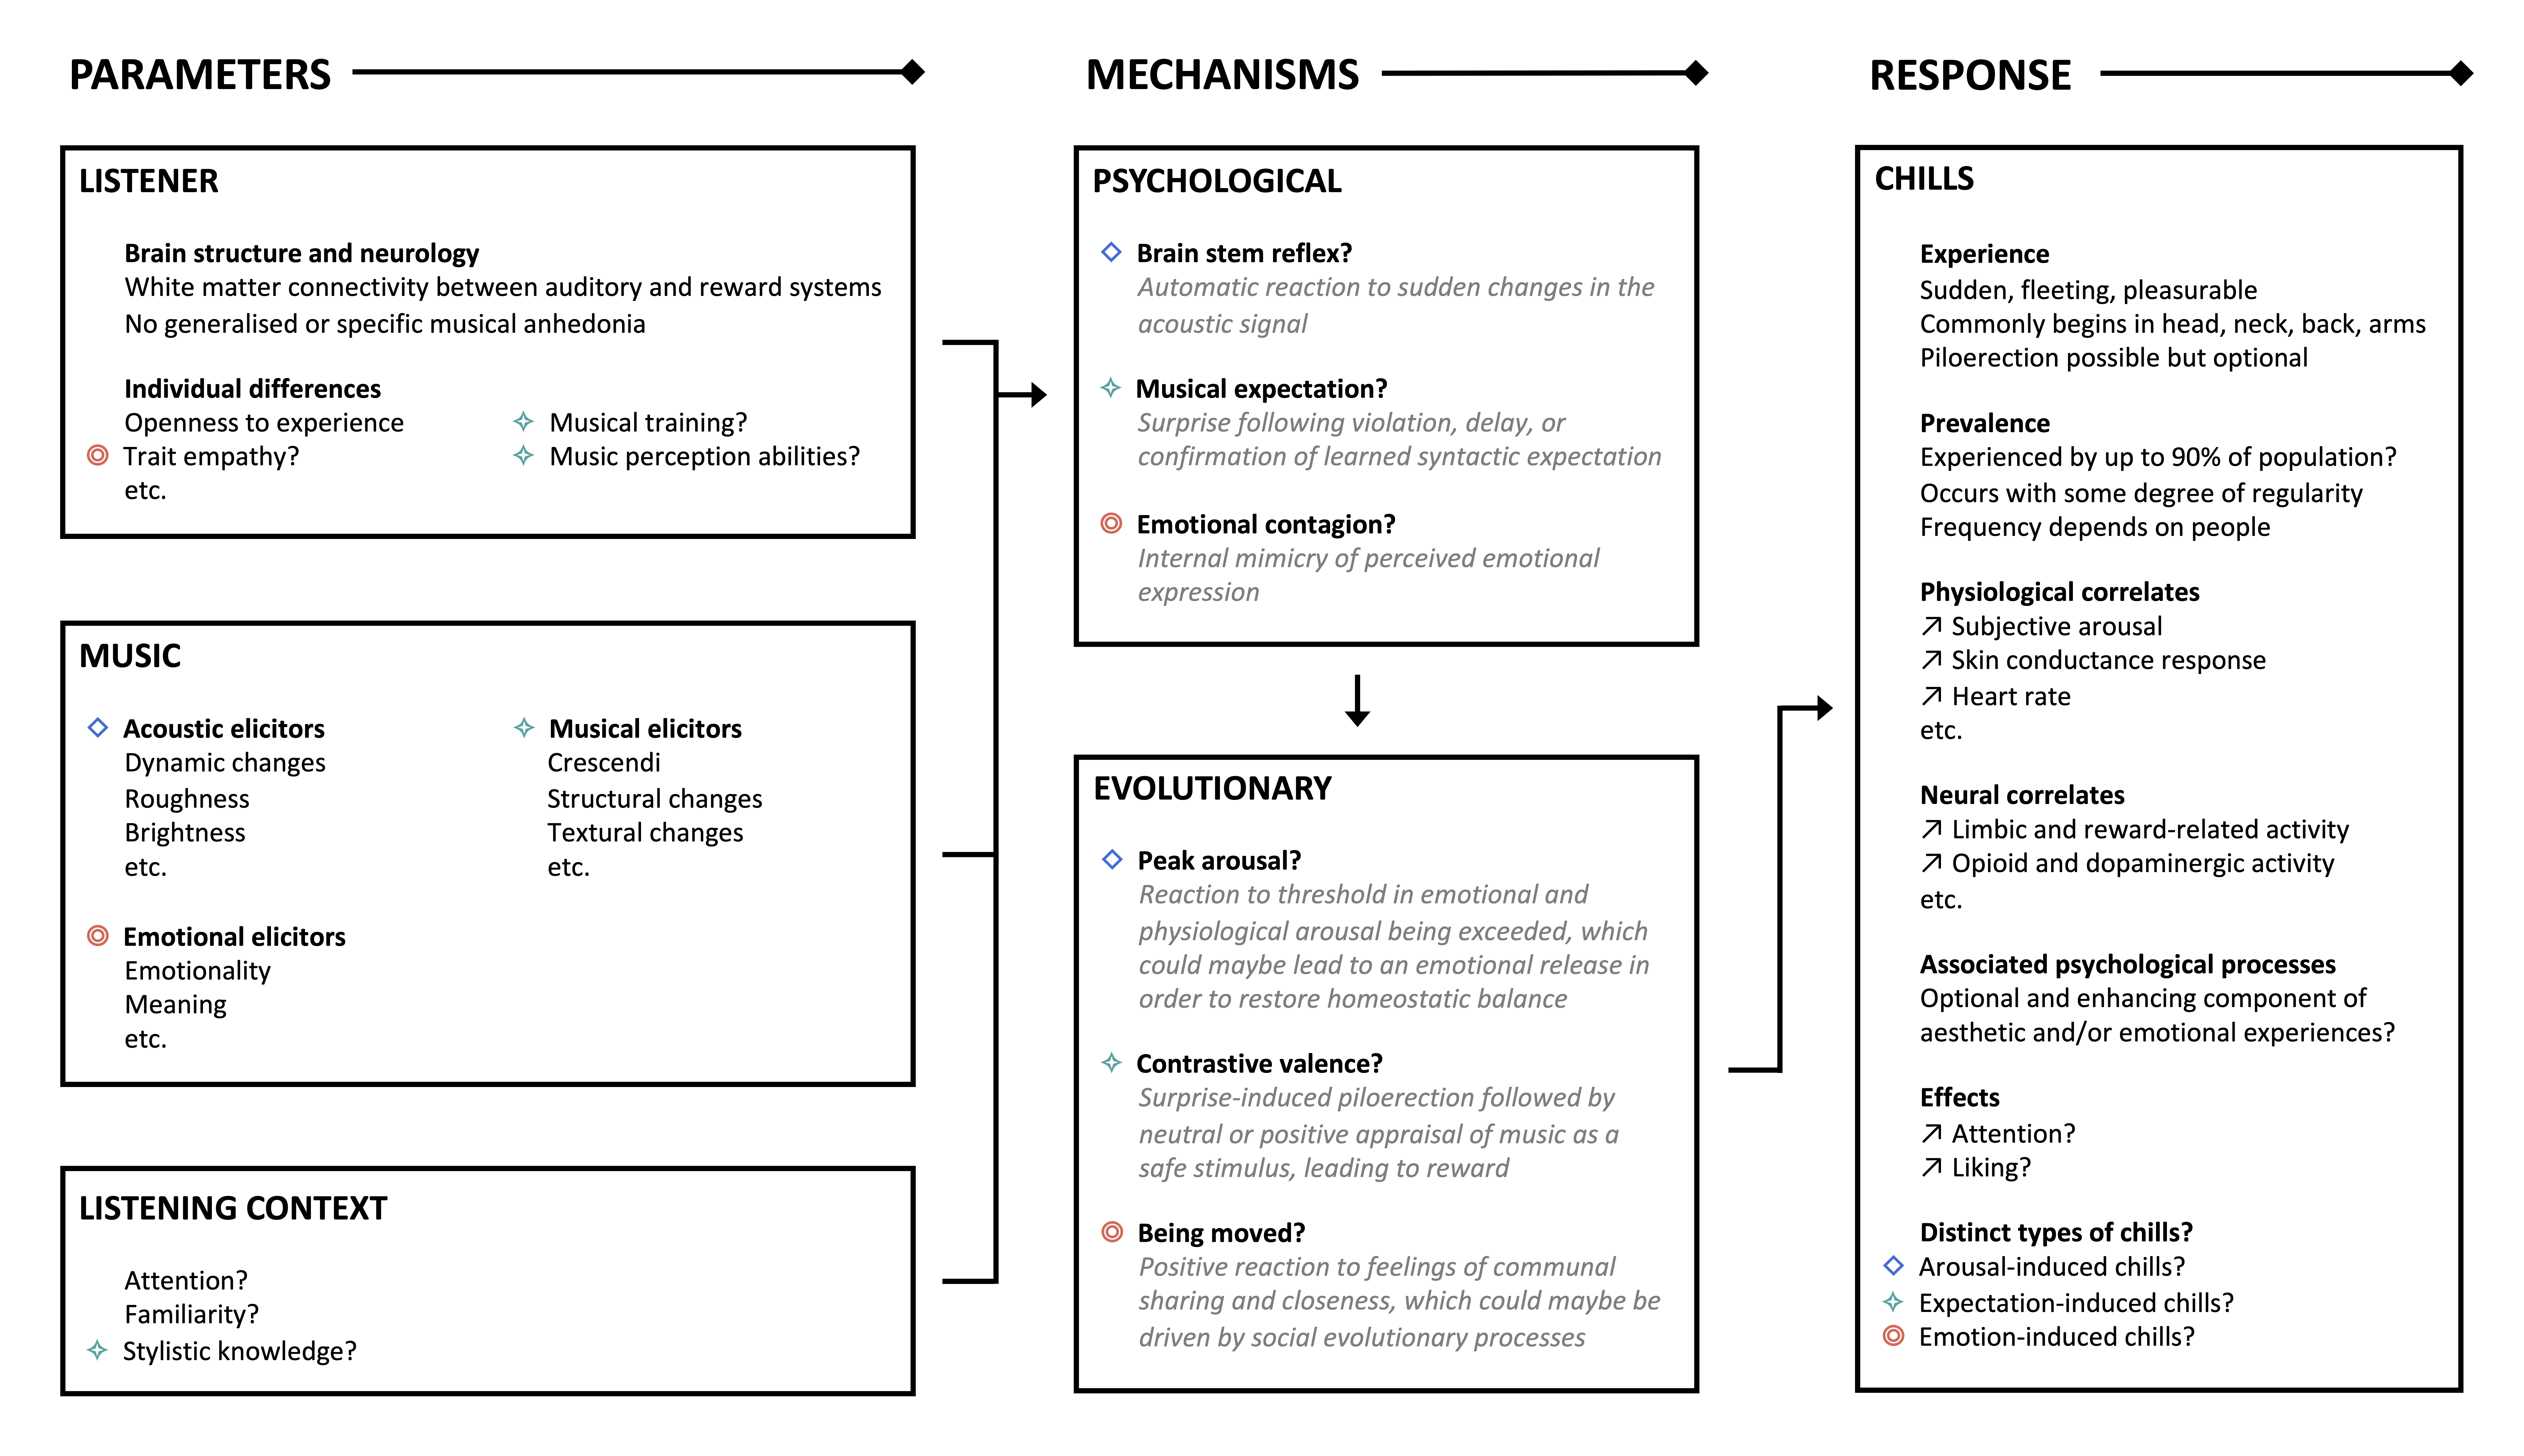
\includegraphics[width=\textwidth]{rev-2.png}
\centering
\caption{Preliminary model of MECs. Parameters on the left represent factors which influence the response of MECs on the right, via psychological and evolutionary mechanisms in the middle. Diagonal arrows represent increases in the associated response. Sentences in italics represent definitions for the listed mechanisms. Question marks represent open questions which lack empirical corroboration. The term ``etc.'' indicates categories for which future evidence or replication of current evidence may warrant the addition of further entries. Symbols link together phenomena which could be related, and could contribute to distinct experiences of MECs.}
\label{fig:rev-2}
\end{figure}

\subsubsection{Dataset of MECs}

Empirical studies of music-evoked emotions most often feature stimuli pertaining to MECs \parencite{warrenburg2020}, such that a large quantity of music which can cause MECs has been documented in the academic literature on MECs. With the aim of facilitating more integrated research on MECs, we have compiled \emph{Chills in Music (ChiM)}, a dataset which contains, to our knowledge, all pieces of music which have been reported to elicit MECs in the literature reviewed in the present chapter\footnote{ChiM is available at \url{https://doi.org/10.17605/osf.io/uyg7m}.}. Details about the preparation of ChiM are available in Chapter \ref{ch:4}. It should be noted that the dataset contains little information about the timing of MECs in most pieces of music, due to limited information in the reviewed literature. Efforts should be expanded to augment ChiM with precise timing information, in order to support future computational research on MECs.

\subsubsection{Open issues and recommendations}

In this section, we highlight open issues in the literature on MECs, based on the reviewed literature and on the preliminary model presented above. In our view, investigating these issues has the most potential to advance research on MECs. Throughout this systematic review, we also identified significant methodological shortcomings regarding research design, adequacy of experimental variables, measures of MECs, and terminology. We provide suggestions for addressing these shortcomings below.

\autoref{tab:rev-7} lists what we consider to be the most important open issues in the available evidence on MECs, along with hypotheses and recommended experimental approaches. While all these issues are derived from the model of MECs we provided, we make a distinction between issues arising from the reviewed literature, and specific predictions arising from the proposed model.

\begin{table}[t!]
\centering
\tiny
\def\arraystretch{1.2}

\begin{threeparttable}
\caption{Open issues, hypotheses, and suggested approaches}
\label{tab:rev-7}

\begin{tabular*}{\textwidth}{
    >{\raggedright}p{0.1\textwidth}
    >{\raggedright}p{0.24\textwidth}
    >{\raggedright\arraybackslash}p{0.555\textwidth}}

\hline

\textbf{Open issue} & \textbf{Hypothesis} & \textbf{Suggested approach} \\ 

\hline
Universality of chills & 
    MECs are experienced by the same proportion of the population, regardless of culture, but are dependent on enculturation. &
    Conduct a large-scale, cross-cultural survey of MECs, recording information about exposure to various musical cultures and genres. \\ 

\hline
Occurrence of piloerection &
    Piloerection occurs once MECs exceed an intensity threshold. &
    Record self-reported intensity of MECs and compare to measured piloerection. This might require further validation or development of piloerection sensors. \\
  
\hline  
Specificity of MECs &
    MECs exhibit different physiological and neural signatures than those of emotion or pleasure. &
    Compare responses with self-selected music that can elicit distinct experiences of MECs, emotion, and pleasure. If there is specificity, a classifier could be trained to distinguish unlabelled instances of MECs from emotional and pleasurable episodes without MECs. \\
    
\hline 
Acoustic and musical elicitors &
    The effect of acoustic elicitors on MECs is partially mediated by musical elicitors, and vice versa. &
    Compare extracted acoustic and musical features (using music information retrieval and/or manual annotation) around the onset of MECs (using a dataset such as the one provided in this review). Alternatively, systematically manipulate stimuli to independently vary the two types of elicitors and compare occurrences of MECs. \\
    
\hline
Familiarity &
    MECs are experienced more frequently as familiarity increases. &
    Use a longitudinal design to study the progress of the frequency of MECs when repeatedly exposed to previously unfamiliar and familiar music with the potential to elicit MECs. \\
    
\hline
MECs and attention &
    Attending to music increases the likelihood of MECs occurring, and MECs focus attention towards the eliciting music. &
    Assess the occurrence of MECs at rest and during a non-musical distractor task while listening to music. Fewer MECs should occur while distracted, and if they occur, they should impair performance on the task. \\
    
\hline
Psychological mechanisms &
    Exploratory animal and developmental research can help pinpoint the psychological and neural mechanisms underlying MECs. &
    Since brain stem reflex, musical expectation, and emotional contagion rely on different psychological and neural mechanisms, which might be more or less well developed in different species and at different developmental stages, exploring the prevalence of MECs in animals and individuals varying in developmental age could shed light on the mechanisms underlying MECs, and identify developmental trajectories. \\
    
\hline
Peak arousal &
    MECs can occur in response to peaks in arousal or pleasure, but might not always since several mechanisms drive the occurrence of MECs. &
    Record measures of physiological arousal for a large number of MECs to identify a threshold for peak arousal or subjective pleasure. MECs should happen every time this threshold is exceeded, but could also happen below this threshold if elicited by a different mechanism. \\
    
\hline
Musical expectation &
    MECs can occur in response to violations of expectation, but might not always since several mechanisms drive the occurrence of MECs. &
    Collect precise timing information for when MECs occur (or use the dataset provided in this review), and compare them to the output from a computational model of expectation. MECs should always occur for sufficiently strong violations of expectation but might occur elsewhere if elicited by a different mechanism. \\

\hline    
Evolutionary mechanisms* &
    MECs can occur via either peak arousal, contrastive valence, or the process of being moved. &
    Carefully prepare stimuli with the potential to elicit MECs via these three mechanisms, controlling for the others, and collect continuous measures (for instance, the two measures detailed above for peak arousal and expectation, and self-reports for being moved). Peaks for each measure should correspond to the onset of MECs for each targeted mechanism. \\

\hline    
Listener and context* &
    Susceptibility to MECs caused via different mechanisms is partly governed by individual differences, familiarity, and stylistic knowledge. &
    Using the approach detailed above, compare individual differences and personality correlates across participants who reported the most MECs for each mechanism. Include familiarity and stylistic knowledge for each piece of music as a random effect in a mixed effect model. \\

\hline    
Distinct types of MECs* &
    Different parameters and mechanisms cause different types of MECs, with distinct physiological and neural signatures. &
    Similarly, using the approach detailed above, compare physiological and neural correlates for MECs elicited via each mechanism. Alternatively, collect these measures along with qualitative descriptions of MECs to identify differences between different categories of MECs. \\
    
\hline

\end{tabular*}
\begin{tablenotes}
\footnotesize
\item Note. * Predictions derived from preliminary model of MECs.
\end{tablenotes}
\end{threeparttable}
\end{table}

Throughout this chapter, we have provided methodological recommendations to address shortcomings in the research on MECs. Notably, we recommended that piloerection should not be used as the sole indicator of MECs, that MECs should not be used as the sole indicator of emotional and aesthetic responses, and that individual differences should be taken into account, particularly because chills could be a multi-faceted phenomenon, which could lead to null, conflicting, or misleading results if this is not taken into consideration. We argued that a combination of self-reports and objective measures are currently best suited for the study of MECs, and that care should be taken when validating self-reports of MECs with skin conductance response. Finally, we recommended the use of the terms chills and piloerection, and suggest a definition for participants in research on MECs, characterising MECs as a fleeting, pleasurable bodily sensation, sometimes accompanied by goosebumps, experienced when listening to specific musical passages.

\subsection{Conclusion}

We conducted a systematic review of the literature on MECs. Theoretical and empirical findings were integrated, leading to the conclusion that MECs are a prevalent psychophysiological response which can include piloerection, and a pleasurable, though not essential, component of emotional and aesthetic experiences. They have been studied using both subjective and objective measures, with a recent focus on causal approaches---a necessary endeavour due to most of the evidence being correlational in nature, and therefore often difficult to interpret. In terms of biological basis, MECs are associated with physiological changes and increased arousal, and recruit brain structures and systems relevant to emotion, reward, and motivation. We reviewed many possible causes of MECs in this chapter. In light of the quality and quantity of the evidence, we believe certain factors to be of particular importance. Notably, MECs can be elicited by acoustic, musical, and emotional stimulus-driven properties which, taken together, suggest a prominent role of sudden changes in acoustic properties, of high-level structural prediction, and of emotionality. They are influenced by personality differences, and especially openness to experience, which is a strong predictor of the ability to experience MECs. Finally, the more convincing theoretical accounts of the function of MECs suggest an involvement of mechanisms based on expectation, peak emotion, and being moved.

We concluded this chapter by establishing a preliminary framework for future research on MECs, providing a set of minimum criteria for a response to music to be considered as an instance of MECs, a model of MECs that explicitly allows for different psychological pathways for the experience of MECs and different types of MECs, a dataset of pieces of music known to cause MECs, and a list of open issues, hypotheses, and potential experiment approaches.
